% presentation
\documentclass{beamer}

% handout
%\documentclass[handout]{beamer}

%\includeonly{preface}

\mode<beamer>{
  \usetheme{Frankfurt}
  \mode<presentation>
}

\mode<handout>{
  \usepackage{pgfpages}
  \pgfpagesuselayout{2 on 1}[a4paper]
}

\usepackage{tikz}
\usetikzlibrary{mindmap,trees}

% other themes
%\usepackage{beamerthemeWarsaw}
%\usepackage{beamerthemeBoadilla}
%\usepackage[compress]{beamerthemeSingapore}


% layout settings
\setbeamertemplate{blocks}[rounded][shadow=false]
\setbeamertemplate{navigation symbols}{}
\setbeamersize{text margin left = 4mm}
\setbeamersize{text margin right = 4mm}
\setbeamercovered{transparent}

% other packages
%\usetheme[Boadilla]{}
\usepackage{calc}
\usepackage[ruled]{algorithm2e}
\usepackage{stmaryrd}
%

%\usepackage{tabularx,booktabs}
\usepackage{booktabs}
%\useinnertheme{rounded}
\usecolortheme{dolphin}
\usecolortheme{rose}
%\setbeamercolor{title}{fg=black,bg=white!80!black}
\setbeamercolor{title}{fg=black,bg=white!80!blue}
\usefonttheme[onlysmall]{structurebold}


\usepackage{colortbl,fancyvrb}

\usepackage{listings}


\definecolor{lightgray}{gray}{0.9}
\definecolor{lightergray}{gray}{0.92}
\definecolor{mygreen}{rgb}{0.1,0.9,0.3}

\definecolor{mydarkgray}{rgb}{0.25,0.3,0.25}
\lstset{
  language=Matlab,
  escapeinside="",
  keywordstyle=\color{black},
  numbersep=5pt,
	framexleftmargin=5pt,
	framexrightmargin=5pt,
	framextopmargin=10pt,
	framexbottommargin=10pt,
  moredelim=[is][\color{gray}\itshape]{/*}{*/},
	moredelim=[is][\alert]{/+}{+/},
  fancyvrb=true
}



\lstdefinestyle{input}{
	frame=leftline,
	framerule=2pt,
	rulecolor=\color{mygreen},
	backgroundcolor=\color{lightgray},
	basicstyle=\smaller\color{black}}

\lstdefinestyle{output}{
	frame=leftline,
	framerule=2pt,
	rulecolor=\color{gray},
	backgroundcolor=\color{lightergray},
	basicstyle=\scriptsize\ttfamily\color{darkgray},
	emph={ODF,Miller,PoleFigure,Symmetry},emphstyle={\color{blue}\underbar}}



\newtheorem{Remark}{Remark}
\newtheorem{Proposition}{Proposition}
\renewcommand{\O}{\mathcal O}
\newcommand{\PGroup}{S_\text{Point}}
\newcommand{\Y}{\mathcal Y}
\renewcommand{\angle}{\measuredangle}
\newcommand{\mtex}{{\large \bf{\color{red}M}TEX\,}}%
\newcommand{\MTEX}{{\bf {\color{red}M}TEX\,}}%
\newcommand{\degree}{\ensuremath{^\circ}}   % Gradzeichen
%\newcommand{\degree}{^\circ}
\newcounter{exercisescounter}
\newenvironment{Exercise}{\refstepcounter{exercisescounter}%
  \begin{block}{Exercise \arabic{exercisescounter}}}
  {\end{block}}


\author{R. Hielscher}

\title{{\Huge \bf{\color{red}M}TEX}}
\subtitle{A Texture Calculation Toolbox}
%\titlegraphic{\includegraphics[width=1.5cm]{pic/tu_logo}}

\institute{Faculty of Mathematics,\\
	Chemnitz University of Technology, Germany}

\date{Prag, 30.5. -- 2.6. 2011}


\begin{document}


\frame[plain]{\titlepage}

\mode<handout>{
 \frame[plain]{}
}

\section{MTEX}


\begin{frame}{What is \MTEX: some numbers and facts}


\begin{block}{}

%\mindmap?
\begin{itemize}
\item developed since 2007
\item 25000 lines of matlab code in over 900 m-files
\item 15000 lines comments
\item 750 help pages
\item 5 reference papers
\item support for 20 pole figure and 5 EBSD data formats
\end{itemize}
\end{block}

\begin{block}{}
  \vspace*{0.25em}
  \hspace{1.25em}
  \begin{tabular}{lll}
    version & release date & downloads \\
    \toprule
    mtex 1.0 & June 2008 & $900$ \\
    mtex 2.0 & October 2009 & $800$ \\
    mtex 3.0 & August 2010 & $650$\\
    mtex 3.2 & May 2011 &
  \end{tabular}
\end{block}


\end{frame}



\begin{frame}
  \frametitle{Feature Overview}

 \renewcommand{\arraystretch}{1.25}
 \begin{center}

  \begin{tabular}{p{3cm} p{8cm}}
    Classes & Methods \\
    \toprule
    \rowcolor{blue!10}
    Crystal Geometry & crystal symmetries, CIF files, Miller indices, Euler angles, orientations,
    missorientations\\
    ODF & model ODFs, pole figures, inverse pole figures, volume portions,
    modal orientations, texture index\\
    \rowcolor{blue!10}
    Pole Figures & outliers, ODF estimation, error analysis\\
    EBSD  & orientation statistics, ODF estimation, grain detection,
    missorientation analysis\\
    \rowcolor{blue!10}
    Grains & volume, surface, neighbors, mean orientation, missorientation\\
    Tensors& elasticity tensors, Young's
    modulus, shear modulus, Poisson's ratio, linear compressibility,
    wave velocities
  \end{tabular}
  \end{center}
 \end{frame}


%%% Local Variables:
%%% mode: latex
%%% TeX-master: "main"
%%% End:


%\section{MATLAB}

\subsection*{Vectors and Matrixes}


\begin{frame}[fragile]
  \frametitle{Vectors and Matrixes}

Define vectors:

\begin{lstlisting}
v = [1;2;3;4];     % a vertical vector
h = [1 2 3 4];     % a horizontal vector
M = [[1;2] [3;4]]; % a 2x2 Matrix
s = 1:4;           % the same as h
\end{lstlisting}

Calculate with vectors:
\begin{lstlisting}
u = 5 * v    % multiply vectors by a scalar
w = u - v    % subtract two vectors
x = u .* v   % componentwise multiplication
y = [u v]    % concatenation of vectors
\end{lstlisting}

Example: polar to Euclidean coordinates
\begin{lstlisting}
x = sin(theta) .* cos(rho)
y = sin(theta) .* sin(rho)
\end{lstlisting}

\end{frame}

\subsection*{Indexing of Vectors}

\begin{frame}[fragile]
  \frametitle{Vectors}


Indexing by numbers:

\begin{lstlisting}
v(1)     % the first element
v(2:end) % the last three elements
M(2,1)   % the bottom left element
M(:,2)   % the second column
\end{lstlisting}

Indexing by conditions:

\begin{lstlisting}
v( v > 1 )   % all elements that are larger then 1
v( u == v)   % all elements where u and v coincides
\end{lstlisting}

Changing elements

\begin{lstlisting}
v(1:3) = 1       % set the first three elements to 1
v( v == 0 ) = [] % remove all zeros
\end{lstlisting}

\end{frame}

\subsection*{Working with Data}


\begin{frame}[fragile]
  \frametitle{A First Script}

Load raw pole figure data stored in a column formated ascii file and plot the
data as colorcoded circles.

\begin{lstlisting}
uiimport([mtexDataPath '/juelich/104.hem']);

theta = data(:,1);     % first row is polar angle
rho = data(:,2);       % second row is azimuth angle
intensity = data(:,3); % third row is intensity

scatter(rho,theta,50,intensity,'filled') % plot data

\end{lstlisting}

\center{\includegraphics[width=10cm]{pic/scatter}}

\end{frame}


\subsection*{Exercises}

\begin{frame}

  \begin{Exercise}
    \begin{enumerate}[a)]
      \item  Construct a vector \textbf{e} of all even numbers between 10 to 30.
      \item  Construct a vector \textbf{s} of the first 11 sqare numbers.
      \item  Set in \textbf{s} all values to 0 where \textbf{e} $>$ \textbf{s}!
    \end{enumerate}
  \end{Exercise}

  \begin{Exercise}
    \begin{enumerate}[a)]
    \item Load the file \texttt{data/juelich/104.hem} and plot the data as a
      scatter plot!
    \item Determin the minimum, maximum and mean
      intensity of the data!
    \item Plot a histogram of the intensities.
    \item Transform the data into cartesian coordinates and plot them!
    \item Remove all negative values from the data and plot them!
    \end{enumerate}
  \end{Exercise}
\end{frame}



%%% Local Variables:
%%% mode: latex
%%% TeX-master: "main"
%%% End:


\section{Geometry}



\subsection*{Vector3d}

\begin{frame}[fragile]
  \frametitle{Specimen Directions - The \MTEX Class \texttt{\bf vector3d}}

  Definition:

\begin{lstlisting}
v = vector3d(1,1,1);    % by Cartesian coordinate
v = sph2vec(theta,rho); % by polar coordinates
v = xvector;            % predefined vectors
\end{lstlisting}

  \medskip

  \begin{columns}
    \begin{column}{8.5cm}

      Calculations:

\begin{lstlisting}
v = [xvector,yvector]; w = v(1);
v = 2*xvector-yvector;
\end{lstlisting}

    \medskip

    Basic Functions:

\begin{lstlisting}
cross(v1,v2), dot(v1,v2)
norm(v), sum(v)
vec2sph(v)
\end{lstlisting}
  \end{column}
  \begin{column}{3cm}
   \includegraphics[width=3cm]{pic/vector3d}
  \end{column}
\end{columns}



\end{frame}

\subsection*{quaternion}


\begin{frame}[fragile]
  \frametitle{Rotations - The \MTEX Class \texttt{\bf quaternion}}

Definition:

\begin{lstlisting}
q = quaternion(a,b,c,d);
q = axis2quat(axis,omega);
q = euler2quat(alpha,beta,gamma);
q = euler2quat(phi1,Phi,phi2,'Bunge');
q = Miller2quat([h k l],[u v w],CS);
\end{lstlisting}
%q = idquaternion;

\medskip

\begin{columns}
  \begin{column}{8.5cm}

    Calculations:

\begin{lstlisting}
q = [q1,q2]; q1 = q(1)
q = q1 * q2; w = q * v
\end{lstlisting}

    \medskip

    Basic Functions:

\begin{lstlisting}
omega = rotangle(q)
v = rotaxis(q)
[alpha,beta,gamma]  = quat2euler(q)
\end{lstlisting}

  \end{column}

  \begin{column}{3cm}
    \includegraphics[width=3cm]{pic/quaternion}
  \end{column}

\end{columns}
\end{frame}

\subsection*{Symmetry}
\begin{frame}[fragile]
  \frametitle{Crystal Symmetries - The \MTEX Class \texttt{\bf symmetry}}

  Definition:

\begin{lstlisting}
S = symmetry('triclinic',[a,b,c],[alpha,beta,gamma])
S = symmetry('-3m',[a,b,c],/+'a||x'+/);
S = symmetry('O');
\end{lstlisting}

\medskip

\begin{columns}
  \begin{column}{8.5cm}

Load Symmetry from CIF file:

\begin{lstlisting}
cif2symmetry('quartz.cif')
\end{lstlisting}

\medskip

    Basic Functions:

\begin{lstlisting}
symmetriceVec(SS,v)
dist(CS,SS,q1,q2)
quaternion(CS)
getFundamentalRegion(CS)
\end{lstlisting}
  \end{column}

  \begin{column}{3cm}
    \includegraphics[width=3cm]{pic/sym}
  \end{column}

\end{columns}

\end{frame}

\subsection*{Miller}

\begin{frame}[fragile]
  \frametitle{Crystal Directions - The \MTEX Class \texttt{\bf Miller}}

  Definition:

\begin{lstlisting}
h = Miller(1,0,0,CS);
h = [Miller(1,1,-2,3,CS),Miller(0,1,-1,0,CS)]
h = vec2Miller(v,CS);
\end{lstlisting}

\medskip

\begin{columns}
  \begin{column}{8.5cm}

    Calculations:

\begin{lstlisting}
q * Miller(1,0,0,CS)
q * symeq(Miller(1,0,0,CS))
\end{lstlisting}

    \medskip

    Basic Functions:


    \begin{onlyenv}<1>
\begin{lstlisting}
symeq(h1,h2)
symvec(h)
angle(h1,h2)
plot([h1,h2],'all')
\end{lstlisting}
    \end{onlyenv}

    \begin{onlyenv}<2>
      \lstset{stringstyle=\color{red},emph={antipodal},emphstyle=\em\color{red}}
\begin{lstlisting}
symeq(h1,h2,`antipodal`)
symvec(h,`antipodal`)
angle(h1,h2,`antipodal`)
plot([h1,h2],'all',`antipodal`)
\end{lstlisting}
    \end{onlyenv}

  \end{column}

  \begin{column}{3cm}
    \includegraphics[width=3cm]{pic/miller}
  \end{column}

\end{columns}

\end{frame}

\subsection*{S2Grid}


\begin{frame}[fragile]
  \frametitle{Sets of Specimen Directions - The \MTEX Class \texttt{\bf S2Grid}}

Definition:

\begin{lstlisting}
S2G = S2Grid('regular','resolution',5*degree);
S2G = S2Grid('regular','maxrho',80*degree);
S2G = S2Grid('equispaced','points',10000);
\end{lstlisting}

\medskip

Basic Functions:

\begin{lstlisting}
add, delete, rotate, union, subGrid, refine,
GridLength, getResolution, getRho, getTheta,
polar, vector3d
\end{lstlisting}

\onslide<1->
\begin{center}
  \includegraphics[width=2.5cm]{pic/S2Grid1} \quad
  \includegraphics[width=2.5cm]{pic/S2Grid2} \quad
  \includegraphics[width=2.5cm]{pic/S2Grid3} \quad
  \includegraphics[width=2.5cm]{pic/S2Grid4}
\end{center}

\end{frame}

\subsection*{Exercises}

\begin{frame}

  \begin{Exercise}
    Consider trigonal crystal symmetry.

    \begin{enumerate}[a)]
    \item Find all crystallographic directions symmetrically equivalent to $h
      = (1, 0, \bar 1, 0)$ (Miller indices)!
    \item Find crystallographic directions such that the number of their
      crystallographic equivalent directions on the upper hemisphere (without
      equator) is 1, 3, or 6?
    \item Construct an orientation that rotates the crystallographic
      directions $(0,0,0,1)$ and $(2,\bar 1,\bar 1,0)$ onto the specimen
      directions $(1,0,0)$ and $(0,1,0)$, respectively.
    \item Find all crystallographic equivalent orientations to
      $(45\degree,0\degree,0\degree)$ (Euler angle) and give its Euler angles!
    \item Find all crystallographic equivalent specimen directions to the crystal
      direction $(1,1,\bar 2,1)$ under the orientation
      $(45\degree,0\degree,0\degree)$ (Euler angle)!
    \end{enumerate}

  \end{Exercise}

\end{frame}

%%% Local Variables:
%%% mode: latex
%%% TeX-master: "main"
%%% End:


%\section{Model ODFs}


\subsection*{ODFs in MTEX}


\begin{frame}[fragile]
  \frametitle{Orientation Density Functions in \MTEX}


  \centering{
    \includegraphics[width=10cm]{latex_pic/odf}
  }

\end{frame}

\subsection*{ODFs in MTEX}


\subsection*{The Class kernel}


\begin{frame}[fragile]
  \frametitle{The Shape of the ODF -- The \MTEX Class \texttt{\bf kernel}}

Definition:

\begin{lstlisting}
psi = kernel('de la Vallee Poussin',80);
psi = kernel('Abel Poisson','halfwidth',10*degree);
\end{lstlisting}

\medskip

Supported kernel functions:

\begin{quote}
  Abel -- Poisson, de la Vall\'ee Poussin, von Mises -- Fisher, fibre von Mises
  -- Fisher, Gauss -- Weierstrass, Dirichlet, Bump
\end{quote}

Plot of the \textcolor{blue}{Abel Poisson}, the \textcolor{red}{Dirichlet} and
the \textcolor{green}{Bump} kernel:

\onslide<1->
\begin{center}
  \includegraphics[width=3.5cm]{pic/K} \quad
  \includegraphics[width=3.5cm]{pic/RK} \quad
  \includegraphics[width=3.5cm]{pic/Fourier}
\end{center}

\end{frame}

\subsection*{Unimodal ODFs}

\begin{frame}[fragile]
  \frametitle{Defining Unimodal ODFs in \MTEX}

\begin{columns}

  \begin{column}{8.5cm}

      Characteristics of an unimodal ODF:
      \begin{enumerate}
      \item crystal symmetry
      \item specimen symmetry
      \item modal orientation
      \item kernel function
      \end{enumerate}



\begin{lstlisting}
SS = symmetry('orthorhombic')
CS = symmetry('cubic')
q = Miller2quat([1 2 2],[2 2 1],CS);
psi = kernel('von Mises Fisher',...
             'halfwidth',20*degree);
\end{lstlisting}

      \begin{actionenv}<1-| alert@1->
\begin{lstlisting}
odf = unimodalODF(q,CS,SS,psi)
\end{lstlisting}
    \end{actionenv}

\end{column}

    \begin{column}{3cm}
      \onslide<1->
      \includegraphics[width=3cm]{pic/unimodalODF}
    \end{column}
  \end{columns}

\end{frame}



\subsection*{Fibre ODFs}

\begin{frame}[fragile]
  \frametitle{Defining Fibre ODFs in \MTEX}

  \begin{columns}

    \begin{column}{8.5cm}

      Characteristics of an Fibre ODFs:
      \begin{enumerate}
      \item crystal symmetry
      \item specimen symmetry
      \item crystal direction
      \item specimen direction
      \item kernel function
      \end{enumerate}


\begin{lstlisting}
SS = symmetry('triclinic')
CS = symmetry('hexagonal')
h = Miller(1,0,0,CS);
r = xvector;
psi = kernel('Abel Poisson',...
             'halfwidth',18*degree);
\end{lstlisting}

      \begin{actionenv}<1-| alert@1->
\begin{lstlisting}
odf = fibreODF(h,r,CS,SS,psi)
\end{lstlisting}
      \end{actionenv}

\end{column}

    \begin{column}{3cm}
      \onslide<1->
      \includegraphics[width=3cm]{pic/fibreODF}
    \end{column}
  \end{columns}


\end{frame}

\subsection*{Fourier ODFs}

\begin{frame}[fragile]
  \frametitle{Defining Uniform and  Fourier ODFs}

  The uniform ODF:
\begin{lstlisting}
SS = symmetry('triclinic')
CS = symmetry('hexagonal')
\end{lstlisting}

  \begin{actionenv}<1-| alert@1->
\begin{lstlisting}
 odf = uniformODF(CS,SS)
\end{lstlisting}
  \end{actionenv}

  \begin{block}{Fourier expansion of an ODF}
    \begin{equation*}
      f(\vec g) = \sum_{l=0}^L \sum_{k,k'=-l}^l C_l^{k,k'} T_l^{k,k'}(\vec g)
    \end{equation*}
    \begin{equation*}
      C = [C_0,C_1^{-1,-1},C_1^{0,-1},C_1^{1,-1},\ldots,C_1^{1,1},C_2^{-2,-2},\ldots,C_L^{L,L}]
    \end{equation*}
  \end{block}
The Fourier ODF:
  \begin{actionenv}<1-| alert@1->
\begin{lstlisting}
odf = FourierODF(C,CS,SS)
\end{lstlisting}
  \end{actionenv}



\end{frame}

\subsection*{ODF Arithmetic}

\begin{frame}[fragile]
  \frametitle{ODF Arithmetic}


  \begin{columns}
    \begin{column}{6cm}

      Calculate with ODFs:
\begin{lstlisting}
odf1 = unimodalODF(...)
odf2 = fibreODF(...)
odf3 = uniformODF(CS,SS)

odf = 0.2*odf1 + 0.3*odf2
      + 0.5*odf3

\end{lstlisting}

  Rotate ODFs:
\begin{lstlisting}
q = axis2quat(xvector,...
              90*degree);
odf = rotate(odf,q)
\end{lstlisting}


  Standard ODFs:
\begin{lstlisting}
odf = santafee;
\end{lstlisting}


\end{column}
\begin{column}{5cm}
  \includegraphics[width=5cm]{pic/santafeeh}
\end{column}
\end{columns}

\end{frame}

%%% Local Variables:
%%% mode: latex
%%% TeX-master: "main"
%%% End:


\section*{ODF Analysis}

\subsection*{Working with ODFs}

\begin{frame}
  \frametitle{Analyzing and Visualizing ODFs in \MTEX}

  \begin{center}
    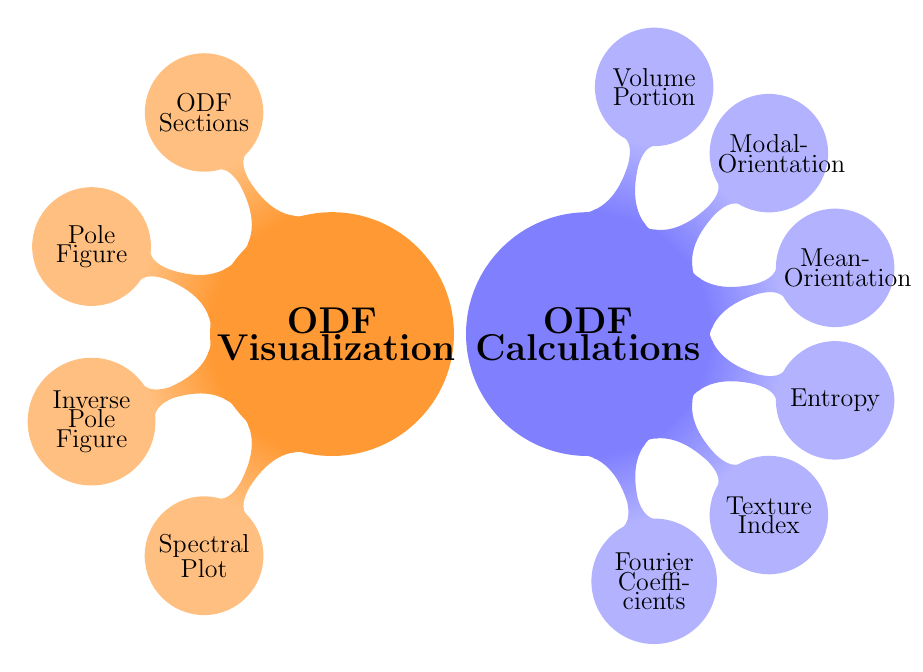
\begin{tikzpicture}[scale = 0.65,transform shape]
  \definecolor{myblue}{HTML}{92dcec}
  \tikzstyle{every annotation}=[fill=white, font=\sf]
  \tikzstyle{root concept}+=[text width=4.5cm]

  \path[mindmap, concept color=orange!80!]
  node[concept] {\huge \bf ODF\\ Visualization}
  child[grow = 120, concept color=orange!50]
  { node(ebsd) [concept](ebsd2) {\Large ODF Sections}}
  child[grow = 160, concept color=orange!50]
  { node[concept](pf) {\Large Pole Figure}}
  child[grow = -160, concept color=orange!50]
  { node[concept](pf) {\Large Inverse Pole Figure}}
  child[grow = -120, concept color=orange!50]
  { node[concept](pf) {\Large Spectral Plot}};

  \path[mindmap, concept color=blue!50!]
  node[concept] at (5,0){\huge \bf ODF \\Calculations}
  child[grow=75, concept color=blue!30]
  { node(ebsd) [concept](ebsd2) {\Large Volume Portion}}
  child[grow=45, concept color=blue!30]
  { node[concept](pf) {\Large Modal\-Orientation}}
  child[grow=15, concept color=blue!30]
  { node[concept](pf) {\Large Mean\-Orientation}}
  child[grow=-15, concept color=blue!30]
  { node[concept](pf) {\Large Entropy}}
  child[grow=-45, concept color=blue!30]
  { node[concept](pf) {\Large Texture Index}}
  child[grow=-75, concept color=blue!30]
  { node[concept](pf) {\Large Fourier Coefficients}};
\end{tikzpicture}
\end{center}

\end{frame}

\subsection*{Working with ODFs}

\begin{frame}[fragile]
  \frametitle{Texture Characteristics}

Comparing {\bf arbitrary} ODFs
\begin{lstlisting}
calcerror(odf1,odf2,'L1')  % 'RP', 'L2'
\end{lstlisting}


\pause

Preferred orientations:
\begin{lstlisting}
o = modalorientation(odf)  % the modal orientation
o = max(odf,n)             % find n relative peaks
o = mean(odf)              % the mean orientation
\end{lstlisting}


\pause

Volume portions:
\begin{lstlisting}
volume(odf,center,radius)   % the volume of a ball
fibrevolume(odf,h,r,radius) % the volume of a fibre
\end{lstlisting}

\pause

The shape of the ODF:
\begin{lstlisting}
textureindex(odf)          % the texture index
entropy(odf)               % the entropy
fourier(odf,order)         % the C-coefficients
\end{lstlisting}


\end{frame}


\subsection*{Plotting (Inverse) Pole Figures}

\begin{frame}[fragile]
  \frametitle{Plotting (Inverse) Pole Figures in \MTEX}

  General syntax:
\begin{lstlisting}
plotpdf(odf,Miller(0,1,0),<options>)
plotipdf(odf,[xvector,zvector],<options>)
\end{lstlisting}

Options:
\begin{lstlisting}
antipodal % add antipodal symmetry
complete  % plot complete sphere
\end{lstlisting}


\onslide<1->
\center{\includegraphics[height=3cm]{pic/ipdf}}

\end{frame}


\subsection*{Plotting an ODF}

\begin{frame}[fragile]
  \frametitle{Plotting  an ODF in \MTEX}

  \begin{columns}
    \begin{column}{6.5cm}
      General syntax:
\begin{lstlisting}
plot(odf,<options>)
\end{lstlisting}

      Sectioning:
      \lstset{emph={sigma},emphstyle={\color{blue}}}
\begin{lstlisting}
alpha, gamma, phi1, phi2
sigma, fibre
\end{lstlisting}

      Options:
\begin{lstlisting}
sections, center, resolution
\end{lstlisting}

      Example:
    \end{column}
    \begin{column}{5cm}
      \includegraphics[width=5cm]{pic/radialplot}
    \end{column}
  \end{columns}

\begin{lstlisting}
plot(odf,'fibre',{Miller(0,0,1),zvector},...
  'center',modalorientation(odf))
\end{lstlisting}

%\begin{lstlisting}
%plot(odf,'alpha',[45*degree])
%\end{lstlisting}

\end{frame}


\subsection*{Dubna}

\begin{frame}[fragile]
  \frametitle{A Sigma Plot of the Recalculated Dubna ODF in \MTEX}

\begin{lstlisting}
plot(rec,'sections',18,'FontSize',10)
\end{lstlisting}

\medskip

\includegraphics[width=\textwidth]{pic/ODFso9}

\end{frame}

\subsection*{SantaFe}

\begin{frame}[fragile]
  \frametitle{The Classical Plot of the SantaFe ODF in \MTEX}

\begin{lstlisting}
plot(SantaFe,'alpha','sections',18,...
     'projection','plain','gray','contourf')
\end{lstlisting}

\includegraphics[width=\textwidth]{pic/santafee}

\end{frame}

\subsection*{Exercises}

\begin{frame}

  \begin{Exercise}
    \begin{enumerate}[a)]
      \item Construct a cubic unimodal ODF with mode at $[0 0 1](3 1 0)$.
      \item What is its modal orientation in Euler angles?
      \item Plot some pole figures. Are there pole figures with and without
        antipodal symmetry? What about the inverse pole figures?
      \item Plot the ODF in $\sigma$ and $\phi_{2}$ - sections. How many modes
        do you observe?
      \item Compute the volume of the ODF that is within a distance of 10
        degrees of the mode. Compare the result with the uniform ODF.
    \end{enumerate}
  \end{Exercise}

  \begin{Exercise}
    \begin{enumerate}[a)]
    \item Construct a trigonal ODF that consists of two fibres at
      $h_1 = (0,0,0,1)$, $r_{1} = \mathbf{y}$, $h_2 = (1,0,\bar 1,0)$, $r_{2} = \mathbf{x}$.
    \item Do the two fibres intersect?
    \item What is the modal orientation of the ODF?
    \item Plot the ODF in $\sigma$ and $\phi_{2}$ - sections. How many
      fibres do you observe?
    \item Compute the texture index of the ODF.
    \end{enumerate}
  \end{Exercise}

\end{frame}


%%% Local Variables:
%%% mode: latex
%%% TeX-master: "main"
%%% End:


\section{Pole Figures Analysis}

\subsection*{Layout}

\begin{frame}[fragile]
  \frametitle{Experimental Pole Figures in \MTEX}

  \begin{columns}

    \begin{column}{8.2cm}

      Characteristics of a single experimental pole figure in \mtex:
      \begin{enumerate}
      \item crystal symmetry
      \item specimen symmetry
      \item list of specimen directions
      \item (list of superposed) crystal direction(s)
      \item (structure coefficients)
      \item list of diffraction intensities
      \item background radiation intensities (optional)
      \end{enumerate}

    \end{column}

    \begin{column}{3cm}
      \includegraphics[width=3cm]{pic/pf1}\\
      \includegraphics[width=3cm]{pic/pfso9_bg}
    \end{column}


  \end{columns}


\end{frame}


\subsection*{Import Wizard}



\begin{frame}[fragile]
  \frametitle{Importing Pole Figure Data - The Import Wizard}

  Formats supported by \MTEX:

  \begin{columns}

    \begin{column}{4cm}
      \begin{itemize}
      \item Popla: *.EPF
      \item BearTex: *.XPa
      \item Philips: *.txt
      \item generic ascii files
      \end{itemize}
    \end{column}

    \begin{column}{4cm}
       \begin{itemize}
      \item Aachen: *.exp
      \item J\"ulich: *.hem
      \item Geesthacht
      \item Dubna: *.cnv, *.cns
      \end{itemize}
    \end{column}

    \begin{column}{3cm}
       \begin{itemize}
      \item *.nja
      \item *.ptx
      \item *.plf
      \item *.xrdml
      \end{itemize}
    \end{column}

  \end{columns}


  \centerline{\includegraphics[width=6cm]{pic/iw}}
\end{frame}

\subsection*{Construction (high level)}

\begin{frame}[fragile]
  \frametitle{Importing Pole Figure Data Using a Script}

  \begin{columns}
    \begin{column}{8.5cm}

Script generated by the import wizard:

\begin{lstlisting}
CS = symmetry('-3m',[1.2 1.2 3.5]);
SS = symmetry('triclinic');
\end{lstlisting}

\pause

\begin{lstlisting}
pf_files = {'Q(10-10).cnv',...
            'Q(10-11)(01-11).cnv'}

h = {Miller(1,0,-1,0,CS),...
     [Miller(0,1,-1,1,CS),...
      Miller(1,0,-1,1,CS)]}

c = {1,[0.52,1.23]};
\end{lstlisting}

\pause

      \begin{actionenv}<1-| alert@1->
\begin{lstlisting}
pf = loadPoleFigure(pf_files,h,...
       CS,SS,'superposition',c);
\end{lstlisting}
      \end{actionenv}

    \end{column}

    \begin{column}{3cm}
      \includegraphics[width=2.5cm]{pic/pforig}
    \end{column}

  \end{columns}

\end{frame}


\subsection*{Analyze Diffraction Data}

\begin{frame}[fragile]
  \frametitle{Using \MTEX to Analyze Diffraction Data}



Retrieve information from pole figures:
\begin{lstlisting}
I = get(pf,'intensities') % intensities
h = get(pf,'Miller')      % Miller indices
r = get(pf,'r')           % specimen directions
\end{lstlisting}

Basic Statistics:
\begin{lstlisting}
min(pf), max(pf), hist(pf), find_outlier(pf)
\end{lstlisting}

\center{\includegraphics[height=3cm]{pic/hist}}

\end{frame}

\subsection*{Modify Pole Figures}

\begin{frame}[fragile]

  \frametitle{Using \MTEX to Modify Pole Figures}

  \begin{columns}

    \begin{column}{8.5cm}

      Pole figure arithmetics:
\begin{lstlisting}
pf = 2*pf1 + 5*pf2;
pf = [pf1,pf2];
pf = pf([1,3,5]);
\end{lstlisting}

      Pole figure modification:

\begin{lstlisting}
scale(pf,alpha),
union(pf1,pf2),
delete(pf,indices),
rotate(pf,q),
set(pf,'intensities',value,indices)
\end{lstlisting}

      \begin{overprint}

        \onslide<2|handout:1>
        Example:
\begin{lstlisting}
theta = get(pf,'polar');
pf = delete(pf,theta >= 70*degree ...
   & theta <= 75*degree)
\end{lstlisting}
        \onslide<3|handout:0>
        Example:
\begin{lstlisting}
pf = rotate(pf,rotation(...
      'axis',xvector-yvector,'angle',25*degree))

\end{lstlisting}
        \onslide<4|handout:0>
        Example:
\begin{lstlisting}
pf = set(pf,'intensities',1,...
        get(pf,'intensities')<1)
\end{lstlisting}

      \end{overprint}
    \end{column}

    \begin{column}{3.1cm}
      \onslide<1->
      \only<1|handout:0>{%
        \includegraphics[height=7.5cm]{pic/pforig}%
      }%
      \only<2>{%
        \includegraphics[height=7.5cm]{pic/pfdelted}%
      }%
      \only<3|handout:0>{%
        \includegraphics[height=7.5cm]{pic/pfrotated}%
      }%
      \only<4|handout:0>{%
        \includegraphics[height=7.5cm]{pic/pfincreased}%
      }
    \end{column}

  \end{columns}

\end{frame}

\subsection*{PDF - to - ODF Reconstruction}


\begin{frame}[fragile]
  \frametitle{PDF to ODF Reconstruction in \MTEX}

  Syntax:
  \begin{alertenv}
\begin{lstlisting}
odf = calcODF(pf,<options>)
\end{lstlisting}
  \end{alertenv}

Options:
\lstset{emph={bandwidth},emphstyle={}}
\begin{lstlisting}
resolution, kernelwidth, bandwidth
iter_min, iter_max
zero_range
ghost_correction
\end{lstlisting}

\pause

\begin{table}[H]
  \centering
  \begin{tabular}{r r r r}
    \toprule
    resolution & kernelwidth  & bandwidth & time \\
    \midrule
    $10^\circ$  & $13.3^\circ$ & 30  & 3s  \\
    $5^\circ$   & $6.7^\circ$  & 58  & 20s \\
    $2.5^\circ$ & $3.3^\circ$  & 121 & 3min\\
    $1.5^\circ$ & $2^\circ$    & 207 & 20min\\
    \bottomrule
  \end{tabular}
\end{table}

\end{frame}


\subsection*{SantaFe}

\begin{frame}[fragile]
  \frametitle{ODF Reconstruction Without Ghost Correction}

\begin{lstlisting}
rec = calcODF(pf_SantaFe,'RESOLUTION',10*degree,...
              'background',1,'iter_max',6)
\end{lstlisting}

\includegraphics[width=\textwidth]{pic/rec_santafee}

\end{frame}
\subsection*{SantaFe}

\begin{frame}[fragile]
  \frametitle{ODF Reconstruction With Ghost Correction}

\begin{lstlisting}
rec = calcODF(pf_SantaFe,'RESOLUTION',10*degree,...
 'background',10,'iter_max',6,'ghost_correction')
\end{lstlisting}

\includegraphics[width=\textwidth]{pic/rec_santafee_ghost_correction}

\end{frame}


\subsection*{Error Analysis}

\begin{frame}[fragile]
  \frametitle{Error Analysis of Reconstructed ODFs in  \MTEX}

Estimate reconstruction error:
\begin{lstlisting}
e = calcerror(pf,odf,<options>)
\end{lstlisting}

Options:
\begin{lstlisting}
RP, L1, L2
\end{lstlisting}

Difference plot:
\begin{lstlisting}
plotDiff(pf,odf,<options>)
\end{lstlisting}

\center{\includegraphics[height=3cm]{pic/diffpf}}

\vspace{3mm}

\end{frame}

\subsection*{Pole Figure Simulation}

\begin{frame}[fragile]
  \frametitle{Pole Figure Simulation in \mtex}

  \begin{columns}
    \begin{column}{8cm}

      Simulation of pole figure data may help to analyze the error made by ODF
      reconstruction from experimental data.

\begin{lstlisting}
%define a model ODF
odf = SantaFe

% define crystal directions
h = [Miller(1,0,0], Miller(1,1,0)]

% define specimen directions
r = S2Grid('regular','antipodal')

% simulate pole figure data
pf = simulatePoleFigure(odf,h,r)
\end{lstlisting}
    \end{column}

    \begin{column}{4cm}
      \centerline{
      \includegraphics[width=4cm]{pic/simpf}}
    \end{column}

  \end{columns}

\end{frame}

\subsection*{Reconstruction Error}

\begin{frame}
  \frametitle{Reconstruction Error vs. Number of Pole Figures}

  \center{\includegraphics[width=10cm]{pic/pfcorrectness}}

\end{frame}

\subsection*{Exercises}

\begin{frame}

  \begin{Exercise}
    \begin{enumerate}[a)]
    \item Load the pole figure data of a quartz specimen from:
      \texttt{data/dubna}!
    \item Inspect the raw data. Are there problems?
    \item Compute an ODF from the pole figure data.
    \item Plot some pole figures of that ODF and compare them to the measured
      pole figures.
    \item Compute the RP errors for each pole figure.
    \item Plot the difference between the raw data and the calculated pole
      figures. What do you observe?
    \item Remove the erroneous values from the pole figure data and repeat the
      ODF calculation. How do the RP errors change?
    \item Vary the number of pole figures used for the ODF calculation. What
      is the minimum set of pole figures required to obtain a reasonable ODF?
    \end{enumerate}
  \end{Exercise}

\end{frame}


%%% Local Variables:
%%% mode: latex
%%% TeX-master: "main"
%%% End:


\section{EBSD Data Analysis}

\begin{frame}[fragile]
  \frametitle{Single Orientation Meassurments - The class EBSD}

  Data stored in the class \alert{EBSD}

  \medskip

  \begin{columns}


    \begin{column}{6cm}

      basic characteristics:
      \begin{itemize}
      \item crystal symmetry
      \item specimen symmetry
      \item individual orientations
      \item phase information
      \end{itemize}

    \end{column}

    \begin{column}{5.5cm}

      additional properties:
      \begin{itemize}
      \item spatial coordinates
      \item Error
      \item IQ, CI, FIT
      \item ...
      \end{itemize}
    \end{column}
  \end{columns}

  \bigskip

  \begin{columns}
    \begin{column}{8cm}
      \includegraphics[height=3.5cm]{pic/ebsd.pdf}
    \end{column}
    \begin{column}{4cm}
      \includegraphics[width=4cm]{pic/ebsdtriangle.pdf}
    \end{column}
  \end{columns}
\end{frame}

\subsection*{Importing EBSD Data}
\begin{frame}[fragile]
  \frametitle{Importing EBSD Data - The Import Wizard}

  \begin{columns}

    \begin{column}{6cm}
      Formats supported by \MTEX:
      \begin{itemize}
      \item HKL: *.ang
      \item Channel: *.ctf
      \item generic: *.txt, *.xls
      \end{itemize}

    \end{column}

    \onslide<1->

    \begin{column}{6cm}
      \includegraphics[width=6cm]{pic/iw2}
    \end{column}

  \end{columns}

\end{frame}


\begin{frame}[fragile]
  \frametitle{Importing EBSD Data - Using a Script}

Script generated by the import wizard:

\begin{lstlisting}
CS = { symmetry('m-3m'), ...
       symmetry('m-3m') }
SS = symmetry('triclinic');
\end{lstlisting}

\begin{lstlisting}
fname = { [ pathto '85_829grad_07_09_06.txt']};
\end{lstlisting}

\begin{actionenv}<1-| alert@1->
\begin{lstlisting}
	ebsd = loadEBSD(fname,CS,SS,'interface',interf,...
	  'ColumnNames', {'Phase' 'x' 'y' ...},...
	  'Columns', [2 3 4 ...],'Bunge',...
	  'ignorePhase', 0);
\end{lstlisting}
\end{actionenv}

\end{frame}

\subsection*{Visualization}

\begin{frame}[fragile]
  \frametitle{Visualize EBSD Data in \MTEX}

  \begin{columns}
    \begin{column}{8.5cm}

Scatter plots in Rodrigues space or axis angle space

\begin{lstlisting}
  scatter(ebsd)
\end{lstlisting}

\pause

Scatter plots in pole figures, inverse pole figures, or ODF sections


\begin{onlyenv}<1,3- |handout:1>
\begin{lstlisting}
		plotpdf(ebsd,[Miller(0,0,1),...])
		plotipdf(ebsd,vector3d(1,0,0))
		plotodf(ebsd)
\end{lstlisting}
\end{onlyenv}

\begin{onlyenv}<2 |handout:0>
\begin{lstlisting}
		/+plotpdf(ebsd,[Miller(0,0,1),...])+/
		plotipdf(ebsd,vector3d(1,0,0))
		plotodf(ebsd)
\end{lstlisting}
\end{onlyenv}

\pause

Spatial plots of EBSD data

\begin{onlyenv}<1-2|handout:0>
\begin{lstlisting}
plot(ebsd)
plot(ebsd,'colorcoding','ipdf')
plot(ebsd,'property','phase')
plot(ebsd,'property','mad')
\end{lstlisting}
\end{onlyenv}

\begin{onlyenv}<3 |handout:1>
\begin{lstlisting}
/+plot(ebsd)+/
/+plot(ebsd,'colorcoding','ipdf')+/
plot(ebsd,'property','phase')
plot(ebsd,'property','mad')
\end{lstlisting}
\end{onlyenv}

\begin{onlyenv}<4 |handout:0>
\begin{lstlisting}
plot(ebsd)
plot(ebsd,'colorcoding','ipdf')
/+plot(ebsd,'property','phase')+/
plot(ebsd,'property','mad')
\end{lstlisting}
\end{onlyenv}

\begin{onlyenv}<5 |handout:0>
\begin{lstlisting}
plot(ebsd)
plot(ebsd,'colorcoding','ipdf')
plot(ebsd,'property','phase')
/+plot(ebsd,'property','mad')+/
\end{lstlisting}
\end{onlyenv}

      Color-Codings: ipdf, hkl, bunge, ihs, angle, sigma

    \end{column}

    \begin{column}{3.5cm}
      \only<1 |handout:0>{%
      \includegraphics[width=3.5cm]{pic/ebsdscatter}%
      }%
      \only<2|handout:0>{%
      \includegraphics[width=3.2cm]{pic/EBSDpdf}%
      }%
      \only<3|handout:1>{%
      \includegraphics[height=7.5cm]{pic/ebsdsmall}%
      }%
      \only<4|handout:0>{%
      \includegraphics[height=7.5cm]{pic/ebsdphase}%
      }%
      \only<5|handout:0>{%
      \includegraphics[height=7.5cm]{pic/ebsdmad}%
      }%
    \end{column}
  \end{columns}
\end{frame}

\subsection*{Grains Analysis}

\begin{frame}[fragile]
  \frametitle{Grain Analysis with \mtex}



  \begin{columns}
    \begin{column}{8.5cm}

      A grain is defined as a region in which the mis\-orien\-tation of
      at least one neigh\-bour\-ing meas\-ure\-ment\-site is smaller than a choosen threshold

\medskip

      Grain Detection

\begin{lstlisting}
[grains ebsd] = segment2d(ebsd,...)
\end{lstlisting}

      \medskip
      Options:
\begin{lstlisting}
'angle'        % threshold angle
'distance'     % max distance
'augmentation' % bounding box
'unitcell'     % no voronoi
\end{lstlisting}

\medskip

Plot grain boundaries:
\begin{lstlisting}
hold on, plotboundary(grains,/+<options>+/)
\end{lstlisting}

\end{column}
    \begin{column}{3.5cm}
      \includegraphics[height=7.5cm]{pic/ebsdgrains}
    \end{column}
  \end{columns}

\end{frame}


\begin{frame}[fragile]
  \frametitle{Grain Properties}

  \begin{columns}
    \begin{column}{8.5cm}


      Copy EBSD properties to the grains

\begin{onlyenv}<1 |handout:1>
\begin{lstlisting}
grains = copyproperty(grains,ebsd)

/+plot(grains,'property','orientation')+/
plot(grains,'property',phase')
\end{lstlisting}
\end{onlyenv}

\begin{onlyenv}<2- |handout:0>
\begin{lstlisting}
grains = copyproperty(grains,ebsd)

plot(grains,'property','orientation')
/+plot(grains,'property',phase')+/
\end{lstlisting}
\end{onlyenv}

\pause
\pause

Access to Properties
\begin{lstlisting}
phase   = get(grains,'phase')
grains1 = grains(phase == 1)
orient  = get(grains,'orientation')
\end{lstlisting}

Interconnection with EBSD Data
\begin{lstlisting}
[grains ebsd] = link(grains,ebsd)
[ebsd grains] = link(ebsd,grains)
\end{lstlisting}

    \end{column}
    \begin{column}{3.5cm}
      \only<1|handout:1>{%
      \includegraphics[height=7.5cm]{pic/ebsdgrainorientation}%
      }%
      \only<2-|handout:0>{%
      \includegraphics[height=7.5cm]{pic/ebsdgrainsphase}%
      }%
    \end{column}
  \end{columns}

\end{frame}


%
\begin{frame}[fragile]
  \frametitle{Grain Properties: Geometry}

Basic functions on grain geometry
\begin{lstlisting}[basicstyle=\footnotesize]
area,perimeter,centroid,hullarea,hullperimeter,
hullcentroid,aspectratio,shapefactor,borderlength,
deltaarea,equivalentperimeter,grainsize,paris
\end{lstlisting}
%

\begin{columns}[t]
  \begin{column}[T]{6.5cm}
  Grain-Size distribution
\begin{lstlisting}
A = area(grains);
% histogram
bar( hist(A,exp(-1.5:6.5)) )
\end{lstlisting}

Other Properties:
\begin{lstlisting}[basicstyle=\footnotesize]
hasholes,hassubfraction
\end{lstlisting}

	\end{column}
	\begin{column}[T]{5cm}
		\includegraphics[width=5cm]{pic/grh}
	\end{column}
\end{columns}

Selecting grains after properties
\begin{lstlisting}
grains = grains( area(grains) > mean(area(grains)) )
\end{lstlisting}

\end{frame}


%
\begin{frame}[fragile]
  \frametitle{Working with EBSD Data Directly}

	Access EBSD Properties
\begin{lstlisting}
	orientations = get(ebsd,'orientation')
	x = get(ebsd,'x')
\end{lstlisting}

	\medskip

	Rotate EBSD Data
\begin{lstlisting}
	ebsd = rotate(ebsd,rotation(...
			'axis',xvector,'angle',90*degree))
\end{lstlisting}

	\medskip
        Omit one pixel grains
\begin{lstlisting}
%grains containing more than one pixel
grains = grains(grainsize(grains) > 1)

%restrict ebsd data to those grains
ebsd = link(ebsd,grains)
\end{lstlisting}

\end{frame}

\subsection*{EBSD - to - ODF Reconstruction}


\begin{frame}[fragile]
  \frametitle{EBSD to ODF Reconstruction in \MTEX}

  \mtex uses kernel density estimation to compute an ODF from EBSD data. The
  sensitive parameter of this method is the kernel function.

\medskip

  Syntax:
  \begin{alertenv}
\begin{lstlisting}
odf = calcODF(ebsd,<options>)
\end{lstlisting}
  \end{alertenv}

Options:
\lstset{emph={bandwidth},emphstyle={}}
\begin{lstlisting}
'kernel'     % the kernel to be used
'halfwidth'  % halfwidth of the kernel function
'resolution' % resolution of the approximation grid

'Fourier'    % ODF by its Fourier coefficients
'exact'      % no approximation to a corser grid
\end{lstlisting}


\end{frame}

%\subsection*{EBSD Simulation}

\begin{frame}[fragile]
  \frametitle{EBSD Simulation in \mtex}

  Simulation of EBSD data may help to analyze the error made by ODF kernel
  density estimation from experimental data.

\begin{lstlisting}
ebsd = simulateEBSD(santafee,5000)
\end{lstlisting}

Compute the error between the original ODF and the estimated ODF.
\begin{lstlisting}
error = calcerror(santafee,calcODF(ebsd,/+<options>+/))
\end{lstlisting}

      \centerline{
      \includegraphics[width=10cm]{pic/ebsdcorrectness}}

\end{frame}





\begin{frame}[fragile]
  \frametitle{ODF Estimation with respect to grains}


\begin{columns}[t]
\begin{column}[T]{8cm}

Overall Estimation

\begin{lstlisting}
grains = calcODF(grains,...)
\end{lstlisting}

\medskip

Options already known from previous
\begin{lstlisting}[basicstyle=\footnotesize]
'kernel', 'halfwidth', 'resolution'
\end{lstlisting}

\medskip

Compare it with original EBSD Data
\begin{onlyenv}<1|handout:0>
\begin{lstlisting}
/+odf1 = calcODF(ebsd,...)+/
odf2 = calcODF(grains,...)
calcerror(odf1,odf2)
\end{lstlisting}
\end{onlyenv}

\begin{onlyenv}<2|handout:1>
\begin{lstlisting}
odf1 = calcODF(ebsd,...)
/+odf2 = calcODF(grains,...)+/
calcerror(odf1,odf2)
\end{lstlisting}
\end{onlyenv}

\end{column}
\begin{column}[T]{3.5cm}
\only<1 | handout:0>{\includegraphics[width=3.5cm]{pic/odf_gr_e}}
\only<2 | handout:1>{\includegraphics[width=3.5cm]{pic/odf_gr_g}}
\end{column}
\end{columns}

\end{frame}


\begin{frame}[fragile]
  \frametitle{ODF Estimation of Grains}

Estimation of individual Grain-ODFs based on EBSD Data
\begin{lstlisting}
grains = calcODF(grains,ebsd, ...)
grains = calcODF(grains,ebsd_mis2mean,...
									  'property','ODF_mis',...)
\end{lstlisting}

Applying functions on grain-ODFs
\begin{lstlisting}
tindex = grainfun(function_handle,grains,'ODF',...)
tindex = grainfun(@textureindex,grains,'ODF',...)
\end{lstlisting}

\begin{columns}
\begin{column}[T]{3.5cm}
\includegraphics[width=3.5cm]{pic/grtindxhist}
\end{column}
\begin{column}[T]{8cm}
\includegraphics[width=8cm]{pic/grtindx}
\end{column}
\end{columns}

\end{frame}



\begin{frame}[fragile]
  \frametitle{Misorientation}

%To treat Misorientation of every grain requires an assigned orientation
%\begin{lstlisting}
%grains = mean(grains,ebsd)
%\end{lstlisting}

Misorientation based on EBSD Data to its mean

\begin{onlyenv}<1| handout:1>
\begin{lstlisting}
/+ebsd_mis = misorientation(grains,ebsd)+/
\end{lstlisting}
\end{onlyenv}
\begin{onlyenv}<2| handout:0>
\begin{lstlisting}
ebsd_mis = misorientation(grains,ebsd)
\end{lstlisting}
\end{onlyenv}

\begin{uncoverenv}<2->
\medskip
Misorientation to neighboured grains
\begin{onlyenv}<1| handout:1>
\begin{lstlisting}
ebsd_mis = misorientation(grains)
\end{lstlisting}
\end{onlyenv}
\begin{onlyenv}<2| handout:0>
\begin{lstlisting}
/+ebsd_mis = misorientation(grains)+/
\end{lstlisting}
\end{onlyenv}

\end{uncoverenv}

%\medskip
\begin{columns}[t]
\begin{column}[T]{6.25cm}
\medskip
Misorientation Distribution
\begin{lstlisting}
hist(ebsd_mis)
\end{lstlisting}

and density function
\begin{lstlisting}
odf = calcODF(ebsd_mis,...)
\end{lstlisting}

\end{column}
  \begin{column}[T]{5.25cm}
\only<1|handout:1>{\includegraphics[height=3.5cm]{pic/mis}}
\only<2|handout:0>{\includegraphics[height=3.5cm]{pic/mis2}}
\end{column}
\end{columns}

\end{frame}



\subsection*{Exercises}

\begin{frame}

  \begin{Exercise}
    \begin{enumerate}[a)]
    \item Load the EBSD data:
      \texttt{data/ebsd\_txt/85\_829grad\_07\_09\_06.txt}!
    \item Perform grain modelling with a certain threshold!
    \item Plot the EBSD data together with the grain boundaries!
    \item Compute the mean orientation for each grain and visualize it!
    \item Compute and visualize the grain size distribution!
    \item Explore the geometric properties of the grains! Is there any
      relationship between the size and the mad of the grains?
    \end{enumerate}
  \end{Exercise}

  \begin{Exercise}
    \begin{enumerate}[a)]
    \item Estimate an ODF from the above EBSD data.
    \item Visualize the ODF and some of its pole figures!
    \item Explore the influence of the halfwidth on the kernel
      density estimation by looking at the pole figures!
    \end{enumerate}
  \end{Exercise}


\end{frame}

\begin{frame}

  % \begin{block}{Exercises 6}
  %   \begin{enumerate}
  %   \item Start with an arbitrary model ODF!
  %   \item Compute the volume portion of the ODF within a range of $20\degree$
  %     of the modalorientation and compare it to the corresponding volume of
  %     the uniform ODF!
  %   \item Simulate EBSD data from this ODF with 10.000 orientations.
  %   \item Plot pole figures from the EBSD data and compare them with the pole
  %     figures from the model ODF.
  %   \item Compute the volume portion of the estimated ODF within a range of
  %     $20\degree$ of the modalorientation and compare it to model ODF!
  %   \item Perform these investigations for different sample sizes!
  %   \end{enumerate}
  % \end{block}


  \begin{Exercise}
    \begin{enumerate}[a)]
    \item Estimate an overall grain-ODF and compare it with the ODF of
      original EBSD data
    \item Visualize the textureindex of each grain
    \item Compare the intrinsic misorientation of individual grains to its
      texture properties, how does the threshold angle affect this?
    \item Investigate the misorientation of neighbours, how does the threshold
      angle influence it?
    \end{enumerate}
  \end{Exercise}

\end{frame}



%%% Local Variables:
%%% mode: latex
%%% TeX-master: "main"
%%% End:




\setbeamercolor{alerted text}{fg=gray}



\tikzstyle{every picture}+=[remember picture]

\global\long\def\SO#1{\mathrm{SO}\left(#1\right)}
\global\long\def\S#1{\mathbb{S}^{#1}}
\global\long\def\sc#1{#1_{0}}
\global\long\def\vc#1{\boldsymbol{#1}}
\global\long\def\adj#1{\bar{#1}}
\global\long\def\Cn#1{\mathcal{C}_{#1}}
\global\long\def\Cd#1{\mathcal{\tilde{C}}_{#1}}
\global\long\def\Dn#1{\mathcal{D}_{#1}}
\global\long\def\Dd#1{\mathcal{\tilde{D}}_{#1}}
\global\long\def\Tn#1{\mathcal{T}_{#1}}
\global\long\def\Td{\mathcal{\tilde{T}}}
\global\long\def\On#1{\mathcal{O}_{#1}}
\global\long\def\Od{\mathcal{\tilde{O}}}


\global\long\def\Spoint{\mathcal{S}}


\global\long\def\Spointa{\tilde{\mathcal{S}}}


\global\long\def\Glaue{\mathcal{G}_{\textrm{Laue}}^{\Spoint}}


\global\long\def\Glauea{\tilde{\mathcal{G}}_{\textrm{Laue}}^{\Spoint}}


\global\long\def\I{\vc I}


\global\long\def\A{\vc A}


\global\long\def\D{\vc D}


\global\long\def\W{\vc W}
\global\long\def\V{\vc V}


\global\long\def\Id{\vc E}


\global\long\def\li{\ell}
\global\long\def\lj{\ell^{\prime}}


%\selectlanguage{english}%
\global\long\def\h#1{\hkl(#1)}
\global\long\def\u#1{\hkl[#1]}
\global\long\def\hs#1{\hkl{#1}}
\global\long\def\us#1{\hkl<#1>}



\section{grain modeling}

\subsection*{Modeling grains}

\begin{frame}[fragile]
  \frametitle{Modeling grains}

\textbf{Input:}
Spatially indexed individual orientations
given as list of tuples $\left(\vc x_{\li},p_{\li},q_{\li}\right),\li=1,\dots,n$
with
\begin{itemize}
\item locations $\vc x_{\li}\in\mathfrak{D}$ bounded to some area $\mathfrak{D}\subset\mathbb{R}^{d}$,
\item phase information $p_{\li}\in\mathbb{N}^{+}$ (includes crystal symmetry),
\item orientations $q_{\li}\in\SO 3$.
\end{itemize}

\textbf{Output:}
A graph based data model representing grains and grain boundaries.

\end{frame}


\begin{frame}[fragile]
  \frametitle{Modeling grains}

\begin{overprint}

\onslide<1>
\begin{center}
\includegraphics[height=0.9\textheight]{fig/voronoi-x}
\par\end{center}

\onslide<2>
\begin{center}
\includegraphics[height=0.9\textheight]{fig/voronoi-b1}
\par\end{center}

\onslide<3>
\begin{center}
\includegraphics[height=0.9\textheight]{fig/voronoi-b1}
\par\end{center}


\onslide<4>
\begin{center}
\includegraphics[height=0.9\textheight]{fig/voronoi-b2}
\par\end{center}

\onslide<5>
\begin{center}
\includegraphics[height=0.9\textheight]{fig/voronoi-b3}
\par\end{center}


\onslide<6>
\begin{center}
\includegraphics[height=0.9\textheight]{fig/voronoi-b4}
\par\end{center}

\onslide<7>
\begin{center}
\includegraphics[height=0.9\textheight]{fig/voronoi-b5}
\par\end{center}

\onslide<8>
\begin{center}
\includegraphics[height=0.9\textheight]{fig/voronoi-b6}
\par\end{center}



\onslide<9>
\begin{center}
\includegraphics[height=0.9\textheight]{fig/voronoi-v1}
\par\end{center}


\onslide<10>
\begin{center}
\includegraphics[height=0.9\textheight]{fig/voronoi-v2}
\par\end{center}




\onslide<11>
\begin{center}
\includegraphics[height=0.9\textheight]{fig/voronoi-v2}
\par\end{center}


\onslide<12>
\begin{center}
\includegraphics[height=0.9\textheight]{fig/voronoi-iom-ad}
\par\end{center}


\onslide<13>
\begin{center}
\includegraphics[height=0.9\textheight]{fig/voronoi-iom-adpm}
\par\end{center}


\onslide<14>
\begin{center}
\includegraphics[height=0.9\textheight]{fig/voronoi-iom-adpmg}
\par\end{center}


\onslide<15>
\begin{center}
\includegraphics[height=0.9\textheight]{fig/voronoi-iom-adpmgs}
\par\end{center}


\onslide<16>
\begin{center}
\includegraphics[height=0.9\textheight]{fig/voronoi-iom-adpmgsb}
\par\end{center}


\onslide<17>
\begin{center}
\includegraphics[height=0.9\textheight]{fig/voronoi-iom-f}
\par\end{center}

\end{overprint}

\end{frame}


\begin{frame}[fragile]
  \frametitle{Modeling grains: algorithm}


% \tikzstyle{na} = [baseline=-.5ex]
\tikzset{Ive/.style ={anchor=base,fill=none},%
         Ied/.style ={anchor=base,fill=none},%
         Idg/.style ={anchor=base,fill=none},%
         Ag/.style ={anchor=base,fill=none},%
         Ad/.style = {anchor=base,fill=none},%
         Ams/.style ={anchor=base,fill=none},%
         Aps/.style ={anchor=base,fill=none},%
         Apg/.style ={anchor=base,fill=none},%
         Apgs/.style ={anchor=base,fill=none}}
\only<2>{\tikzset{Ive/.style ={anchor=base,fill=yellow}}}
\only<3>{\tikzset{Ied/.style ={anchor=base,fill=yellow}}}
\only<9>{\tikzset{Idg/.style ={anchor=base,fill=yellow}}}
\only<11>{\tikzset{Ag/.style ={anchor=base,fill=yellow}}}
\only<4>{\tikzset{Ad/.style ={anchor=base,fill=yellow}}}
\only<6>{\tikzset{Ams/.style ={anchor=base,fill=red!30}}}
\only<7>{\tikzset{Aps/.style ={anchor=base,fill=green!30}}}
\only<14>{\tikzset{Apgs/.style ={anchor=base,fill=blue!30}}}
\only<15>{\tikzset{Apg/.style ={anchor=base,fill=green!30}}}
\begin{overlayarea}{\textwidth}{\textheight}
\begin{enumerate}
\item <1-|alert@5->Voronoi-decomposition resulting in incidence matrix
$\tikz[baseline]{\node[Ive](ive){\ensuremath{\I_{VE}}};},
\tikz[baseline]{\node[Ied](ied){\ensuremath{\I_{ED}}};}$
and adjacency matrix
 $\tikz[baseline]{\node[Ad](aa){\ensuremath{\A_{D}}};}$.\only<2>{ {\footnotesize
\[
\left[\tikz[baseline]{\node[Ive](ve){\ensuremath{\I_{VE}}};}\right]^{i,j}=\begin{cases}
1, & \mbox{if vertex }v _{i}\mbox{ incident to edge }e_{j},\\
0, & \mbox{otherwise}.
\end{cases}
\]
}}\only<3>{ {\footnotesize
\[
\left[\tikz[baseline]{\node[Ied](ed){\ensuremath{\I_{ED}}};}\right]^{j,\li}=\begin{cases}
1, & \mbox{if edge }e _{j}\mbox{ incident to Voronoi-cell }D(\vc{x}_{\li}),\\
0, & \mbox{otherwise}.
\end{cases}
\]
}}\only<4>{ {\footnotesize
\[
\left[\tikz[baseline]{\node[Ad](ad){\ensuremath{\A_{D}}};}\right]^{\li,\lj}=\begin{cases}
1, & \mbox{if Voronoi-cell }D(\vc{x}_{\li})\mbox{ adjacent to Voronoi-cell }D(\vc{x}_{\lj}),\\
0, & \mbox{otherwise}.
\end{cases}
\]
}}
\item <5-|alert@8->Decompose adjacencies $\A_{D}=\tikz[baseline]{\node[Ams](Am){\ensuremath{\A_{D}^{\circ}}};}+\tikz[baseline]{\node[Aps](Ap){\ensuremath{\A_{D}^{\partial}}};}$\only<2>{.}\only<6>{,{\footnotesize
\[
\left[\tikz[baseline]{\node[Ams](am){\ensuremath{\A_{D}^{\circ}}};}\right]^{\li,\lj}=\begin{cases}
1, & \mbox{if }D\left(\vc x_{\li}\right)\mbox{ and }D\left(\vc x_{\lj}\right)\mbox{ adjacent and {\color{red}no\,\ grain boundary}},\\
0, & \mbox{otherwise}.
\end{cases}
\]
}}\only<7>{,{\footnotesize
\[
\left[\tikz[baseline]{\node[Aps](ap){\ensuremath{\A_{D}^{\partial}}};}\right]^{\li,\lj}=\begin{cases}
1, & \mbox{if }D\left(\vc x_{\li}\right)\mbox{ and }D\left(\vc x_{\lj}\right)\mbox{ adjacent and {\color{green}grain boundary}},\\
0, & \mbox{otherwise}.
\end{cases}
\]
}}\only<9->{.}
\item <8-|alert@11->Search components of $\A_{D}^{\circ}$
via depth-first search and determine incidence matrix $\tikz[baseline]{\node[Idg](idg){\ensuremath{\I_{DG}}};}
\subseteq D\times G$\only<9>{,{\footnotesize
\[
\left[\tikz[baseline]{\node[Idg](dg){\ensuremath{\I_{DG}}};}\right]^{\li,m}=\begin{cases}
1, & \mbox{if }D\left(\vc x_{\li}\right)\mbox{ is part of grain }g_{m},\\
0, & \mbox{otherwise}.
\end{cases}
\]
}}\only<10->{.}
\item <10-|alert@13->Represent adjacencies of grains in a matrix $\tikz[baseline]{\node[Ag](aga){\ensuremath{\A_{G}}};}\subseteq G\times G$\only<11>{, {\footnotesize
\[
\left[\tikz[baseline]{\node[Ag](ag){\ensuremath{\A_{G}}};}\right]^{m,m^{\prime}}=\begin{cases}
1, & \mbox{if grain }g_{m}\mbox{ and }g_{m^{\prime}}\mbox{ have a common grain boundary},\\
0, & \mbox{otherwise}.
\end{cases}
\]
}}\only<12>{,{\footnotesize
\[
\left[\A_{G}\right]^{m,m^{\prime}}=\begin{cases}
1, & \mbox{if }\left[\I_{DG}^{\top}\A_{D}^{\partial}\I_{DG}\right]^{m,m^{\prime}}>0,\\
0, & \mbox{otherwise}.
\end{cases}
\]
}}\only<13->{.}
\item <13-|alert@16->Decompose adjacencies $\A_{D}^{\partial}=\tikz[baseline]{\node[Apgs](Apgs){\ensuremath{\A_{D}^{\partial_{\mathrm{sub}}}}};}+\tikz[baseline]{\node[Apg](Apg){\ensuremath{\A_{D}^{\partial_{\mathrm{ext}}}}};}$\only<14>{.}\only<14>{,{\footnotesize
\[
\left[\tikz[baseline]{\node[Apgs](apgs){\ensuremath{\A_{D}^{\partial_{\mathrm{sub}}}}};}\right]^{\li,\lj}=\begin{cases}
1, & \mbox{if }D\left(\vc x_{\li}\right)\mbox{ and }D\left(\vc x_{\lj}\right)\mbox{ adjacent and {\color{blue}sub grain boundary}},\\
0, & \mbox{otherwise}.
\end{cases}
\]
}}\only<15>{,{\footnotesize
\[
\left[\tikz[baseline]{\node[Apg](apg){\ensuremath{\A_{D}^{\partial_{\mathrm{ext}}}}};}\right]^{\li,\lj}=\begin{cases}
1, & \mbox{if }D\left(\vc x_{\li}\right)\mbox{ and }D\left(\vc x_{\lj}\right)\mbox{ adjacent and {\color{green}grain boundary}},\\
0, & \mbox{otherwise}.
\end{cases}
\]
}}\only<16>{.}
\item <16-|alert@17->Compute incidence matrix $\I_{EG}=\I_{ED}\I_{DG}$ and  decompose
$\I_{EG}=\I_{EG}^{\circ}+\I_{EG}^{\partial}$, with $\I_{EG}^{\partial}=\I_{EG}^{\partial_{\mathrm{sub}}}+\I_{EG}^{\partial_{\mathrm{ext}}}$.
\end{enumerate}
\only<17->{\textbf{Output}:\\
$\A_{D}^{\circ},\,\A_{D}^{\partial_{\mathrm{sub}}},\,\A_{D}^{\partial_{\mathrm{ext}}},\A_{G},$\\
$\I_{DG},\,\I_{ED}^{\partial_{\mathrm{sub}}},\,\I_{ED}^{\partial_{\mathrm{ext}}},$\\}
\end{overlayarea}
% have to apply the 'overlay' style.
\begin{tikzpicture}[overlay]
   \path[->]<2> (ve) edge [out=60, in=-150,yellow,line width=2pt] (ive);
   \path[->]<3> (ed) edge [out=60, in=-150,yellow,line width=2pt] (ied);
   \path[->]<4> (ad) edge [out=60, in=-150,yellow,line width=2pt] (aa);
   \path[->]<6> (am) edge [out=60, in=-150,red!30,line width=2pt] (Am);
   \path[->]<7> (ap) edge [out=45, in=-150,green!30,line width=2pt] (Ap);
   \path[->]<9> (dg) edge [out=90, in=-120,yellow,line width=2pt] (idg);
   \path[->]<11> (ag) edge [out=45, in=-150,yellow,line width=2pt] (aga);
   \path[->]<14> (apgs) edge [out=45, in=-150,blue!30,line width=2pt] (Apgs);
   \path[->]<15> (apg) edge [out=45, in=-150,green!30,line width=2pt] (Apg);
\end{tikzpicture}

\end{frame}


\begin{frame}[fragile]
  \frametitle{Modeling grains: algorithm}


\textbf{Benefits ... }
\begin{itemize}
\item Works in 2d and 3d
\item Voronoi-decomposition flexible against not indexed data
\item No interpolation of orientation
\item Explicit data model ensures fast access to adjacencies and incidences.
\item Almost every spatial relationship of EBSD data and its grains can be represented.
\end{itemize}


\textbf{... Disadvantages}
\begin{itemize}
\item Voronoi-decomposition is expensive.
\item Large memory costs to store all adjacencies and incidences.
\end{itemize}

\end{frame}



\subsection*{Modeling grains}

\begin{frame}[fragile]
  \frametitle{Modeling grains}


\begin{overprint}

\onslide<1>

\begin{lstlisting}
mtexdata mylonite
plot(ebsd,'property','phase');
\end{lstlisting}

\begin{center}
\includegraphics[width=\linewidth]{fig/twinsa}
\par\end{center}


\onslide<2>
\begin{lstlisting}
grains = calcGrains(ebsd,'angle',5*degree);
hold on, plotBoundary(grains);
\end{lstlisting}

\begin{center}
\includegraphics[width=\linewidth]{fig/twinsb}
\par\end{center}



\onslide<3>
\begin{lstlisting}
plot(grains,'property','phase')
\end{lstlisting}

\begin{center}
\includegraphics[width=\linewidth]{fig/twinsd}
\par\end{center}


\onslide<4>
\begin{lstlisting}
hold on, plotBoundary(grains,'property',...
   orientation(...));
\end{lstlisting}


\begin{center}
\includegraphics[width=\linewidth]{fig/twinsc}
\par\end{center}

\end{overprint}

\end{frame}



\subsection{Properies of grains}
\begin{frame}[fragile]
  \frametitle{Properties of grains}

\textbf{Incidencies and Adjacencies}
\begin{lstlisting}
get(grains,'I_VF')
get(grains,'I_DG')
get(grains,'I_FG')
get(grains,'I_FDext')
get(grains,'I_FDint')
get(grains,'A_D')
get(grains,'A_G')
\end{lstlisting}

\textbf{Properties}
\begin{lstlisting}
get(grains,'EBSD')
get(grains,'orientation')
get(grains,'orientations')
get(grains,'...')
\end{lstlisting}

\end{frame}




\subsection{Properies of grains}
\begin{frame}[fragile]
  \frametitle{Properties of grains}

\textbf{Geometric properties of grains}
\begin{lstlisting}
area(grains)
perimeter(grains)
diameter(grains)
centroid(grains)
shapefactor(grains)
aspectratio(grains)
equivalentradius(grains)
equivalentperimeter(grains)
principalcomponents(grains)
...
\end{lstlisting}

\textbf{Other properties}
\begin{lstlisting}
grainSize(grains)
hasHole(grains)
isNotIndexed(grains)
\end{lstlisting}

\end{frame}


\subsection{Accessing grains}
\begin{frame}[fragile]
  \frametitle{Acessing grains}

\textbf{Accessing by phase}
\begin{lstlisting}
grains('mineral name')
grains({'fe','mg'})
\end{lstlisting}

\textbf{Accessing grains by indexing or logical expression}
\begin{lstlisting}
grains(1)
grains(1:10)
grains( area(grains) > 100 )
grains(diameter(grains)>10 | perimeter(grains)>10)
grains(diameter(grains)>10 & grains('fe'))
grains(grainSize(grains)>1 & ~grains('notindexed'))
\end{lstlisting}

\textbf{Concatenation of grain}
\begin{lstlisting}
[grains('fe') grains('mg')]
\end{lstlisting}
\end{frame}


\subsection{Correcting EBSD and grains}
\begin{frame}[fragile]
  \frametitle{Correcting EBSD and grains}

\begin{overlayarea}{\linewidth}{8cm}
\only<1-2>{
\begin{center}
\only<1>{\includegraphics[width=\linewidth]{fig/ebsd_correction_1a}}
\only<2>{\includegraphics[width=\linewidth]{fig/ebsd_correction_1b}}
\par\end{center}
\begin{enumerate}
\item <1->Import EBSD.
\item <2-> Reconstruct grains.
\end{enumerate}
% \vspace*{\fill}
}

\only<3-5>{
\begin{center}
\only<3>{\includegraphics[width=\linewidth]{fig/ebsd_correction_1a}}
\only<4>{\includegraphics[width=\linewidth]{fig/ebsd_correction_2b}}
\only<5>{\includegraphics[width=\linewidth]{fig/ebsd_correction_2c}}
\par\end{center}
\begin{enumerate}
\item <3->Import EBSD.
\item <4->Remove badly indexed data and remove non-plausible grains, e.g. '1-pixel' grains.
\item <5->Reconstruct grains.
\end{enumerate}
% \vspace*{\fill}
}

\only<6-9>{
\begin{center}
\only<6>{\includegraphics[width=\linewidth]{fig/ebsd_correction_1a}}
\only<7>{\includegraphics[width=\linewidth]{fig/ebsd_correction_3b}}
\only<8>{\includegraphics[width=\linewidth]{fig/ebsd_correction_3c}}
\only<9>{\includegraphics[width=\linewidth]{fig/ebsd_correction_3d}}
\par\end{center}
\begin{enumerate}
\item <6->Import EBSD.
\item <7->Reconstruct grains.
\item <8->Remove non-plausible data but keep some dummy data.
\item <9->Reconstruct grains again.
\end{enumerate}
% \vspace*{\fill}
}



% Data correction is important!\\
% \textbf{Your first exercise when analysing ebsd: correct it.}}
\end{overlayarea}
\end{frame}



\subsection{Grain boundaries and misorienation}
\begin{frame}[fragile]
  \frametitle{Grain boundaries and misorienation}



\begin{overprint}
\onslide<1>
\textbf{via boundary misorientation angular distribution} %\vspace*{-.45cm}
\begin{lstlisting}
plotAngleDistribution(grains)
plotAngleDistribution(grains('fe'),63)
plotAngleDistribution(grains('fe'),grains('mg'),63)
\end{lstlisting}
\begin{center}
\includegraphics[width=7cm]{fig/grains_angledistribution}
\par\end{center}


\onslide<2>
\textbf{via boundary misorientation axis distribution} %\vspace*{-.45cm}
\begin{lstlisting}
plotAxisDistribution(grains('fe'))
plotAxisDistribution(grains('mg'),...
                         'smooth','antipodal')
plotAxisDistribution(grains('mg'),grains('fe'))
\end{lstlisting}
\begin{center}
\includegraphics[width=.3\linewidth]{fig/grains_axisdistribution_fe}
\includegraphics[width=.3\linewidth]{fig/grains_axisdistribution_mg}
\includegraphics[width=.3\linewidth]{fig/grains_axisdistribution_mg_fe}
\par\end{center}


\onslide<3->
\textbf{via spatial plots}%\vspace*{-.45cm}
\begin{lstlisting}
plotBoundary(grains,'property','angle')
plotBoundary(grains,'property','misorientation')
plotBoundary(grains,'property',...
   orientation(...),'delta',2*degree)
plotBoundary(grains,'property',[2 10]*degree)

\end{lstlisting}
\begin{center}
\only<3>{\includegraphics[width=\linewidth]{fig/grains_boundary_angle}}%
\only<4>{\includegraphics[width=\linewidth]{fig/grains_boundary_misorientation}}%
\only<5>{\includegraphics[width=\linewidth]{fig/grains_boundary_special}}%
\only<6>{\includegraphics[width=\linewidth]{fig/ebsd_boundary_1a}}%
\par\end{center}
\end{overprint}

\end{frame}


\subsection{Grains and interal misorienation}
\begin{frame}[fragile]
  \frametitle{Grains and internal misorienation}



\begin{overprint}
\onslide<1-2>
\textbf{Observe misorientation within a grain} %\vspace*{-.45cm}
\begin{lstlisting}
plot(grains,'property','mis2mean')
plot(grains,'property','mis2mean',...
                    'colorcoding','angle')
\end{lstlisting}
\begin{center}
\only<1>{\includegraphics[width=\linewidth]{fig/grains_mis2mean}}%
\only<2>{\includegraphics[width=\linewidth]{fig/grains_mis2mean_angle}}
\par\end{center}


\onslide<3-5>
\begin{overlayarea}{\linewidth}{10cm}
\textbf{Observe misorientation of grains individually} %\vspace*{-.45cm}

\begin{lstlisting}
singlegrain = findByLocation(grains,[x y])
plotKAM(singlegrain)
spatialProfile(singlegrain,[x1 y1; x2 y2])
\end{lstlisting}
\begin{center}
\vspace*{-.5cm}
\only<3>{\includegraphics[width=\linewidth]{fig/grains_misorientation_1a}}%
\only<4->{\includegraphics[width=\linewidth]{fig/grains_misorientation_1b}}%
\vspace*{-.8cm}
\hspace*{1.4cm}\only<5>{
\includegraphics[width=.7\linewidth]{fig/grains_misorientation_1c}}%
\par\end{center}
\end{overlayarea}
\end{overprint}

\end{frame}




\subsection{Grains and misorienation}
\begin{frame}[fragile]
  \frametitle{Grains and misorienation}

\begin{overprint}
\onslide<1>
\textbf{via boundary misorientation angular distribution} %\vspace*{-.45cm}
\begin{lstlisting}
plotAngleDistribution(grains)
plotAngleDistribution(grains('fe'),63)
plotAngleDistribution(grains('fe'),grains('mg'),63)
\end{lstlisting}
\begin{center}
\includegraphics[width=7cm]{fig/grains_angledistribution}
\par\end{center}

\end{overprint}
\end{frame}

\only<3>{
\begin{lstlisting}
plotBoundary(grains,'property','angle')
plotBoundary(grains,'property','misorientation')
plotBoundary(grains,'property',...
   orientation(...),'delta',2*degree)
\end{lstlisting}
}

% \only<4>{
% \textbf{Analyze via misorientations}
% \begin{lstlisting}
% m = calcMisorientation(grains('fe'),grains('mg'))
% axis(m);
% angle(m)/degree;
% \end{lstlisting}

% \textbf{Your exercise}: \texttt{mtexdata mylonite}
% Classify and plot special boundaries
% }

% \end{overprint}
% \end{frame}



\subsection{Organizing grains hierarchically}
\begin{frame}[fragile]
  \frametitle{Organizing grains hierarchically}


\begin{overprint}
\onslide<1>
\textbf{merging grains with certain misorientation angle}
\begin{lstlisting}
[grains5  I_5]  = merge(grains,5*degree);
[grains10 I_10] = merge(grains5,10*degree);

sum(I_5,2); sum(I_10,2);
sum(I_10*I_5,2);
\end{lstlisting}

\onslide<2->
\textbf{merging grains with special boundary}
\begin{lstlisting}
[grains_csl I_csl] = merge(grains,CSL(3));
[grains_o   I_o  ] = merge(grains,...
             orientation(...),'delta',2*degree);
\end{lstlisting}


\begin{center}
\vspace*{-.5cm}
\only<2>{\includegraphics[width=\linewidth]{fig/grains_merge_1a}}%
\only<3>{\includegraphics[width=\linewidth]{fig/grains_merge_1b}}%
\only<4>{\includegraphics[width=\linewidth]{fig/grains_merge_1c}}%
\only<5>{\includegraphics[width=\linewidth]{fig/grains_merge_1d}}%
\par\end{center}

\end{overprint}
\end{frame}


% \section{Grains}


% \subsection{reconstruction of grains}
% \begin{frame}
%   \frametitle{Reconstruction of grains}

% \end{frame}


% \begin{frame}
%   \frametitle{Accessing grains}




% \end{frame}

% \subsection{grain boundary analysis}

% \subsection{Plotting grain boundaries}
% \begin{frame}
%   \frametitle{Plotting grain boundaries}


% \end{frame}


% \begin{frame}
%   \frametitle{misorientation at grain boundaries}




% \end{frame}



% \subsection{Merging grains}
% \begin{frame}
%   \frametitle{Organizing grains}

% merge


% \end{frame}




\subsection{Exercises}
\begin{frame}
  \frametitle{Exercises}

 Examine the EBSD data \textcolor{blue}{\texttt{mtexdata aachen}}:
  \begin{itemize}
  \item Correct the EBSD data / grains.
  \item How does the correction influence the data analysis?
  \end{itemize}

 Examine the EBSD data \textcolor{blue}{\texttt{mtexdata mylonite}}:

  \begin{itemize}
  \item Characterize special grain boundaries for all phases.
  \item Visualize your results.
  \end{itemize}

  Examine the EBSD data \textcolor{blue}{\texttt{ebsd\_mergeCSL3.txt}}:

  \begin{itemize}
  \item Which texture is present?
  \item Characterize special grain boundaries.
  \item Merge grains and investigate merged regions.
  \item What is wrong with the data?
  \end{itemize}


\end{frame}


% \begin{frame}

% \begin{center}
% \includemovie[poster,toolbar,label=grains_vox,text=(5 largest grains),3Dviews2=pic/views.txt,3Djscript=pic/grains_explode.js]{11cm}{8cm}{pic/grains_vox.u3d}
% \end{center}

% \end{frame}



%  \begin{frame}

% \begin{center}
% \includemovie[poster,toolbar,label=grains_smooth,text=(5 largest grains),3Dviews2=pic/views.txt,3Djscript=pic/grains_explode.js]{11cm}
% {8cm}{pic/grains_smooth.u3d}
% \end{center}

%  \end{frame}


% \begin{frame}

% \begin{center}
% \includemovie[poster,toolbar,label=grains_smooth2,text=(5 largest grains),3Dviews2=pic/views.txt,3Djscript=pic/grains_explode.js]{11cm}{8cm}{pic/grains_smooth2.u3d}
% \end{center}

% \end{frame}



%%% Local Variables:
%%% mode: latex
%%% TeX-master: "main"
%%% End:


% presentation
\documentclass[compress]{beamer}

% handout
%\documentclass[handout]{beamer}

\usepackage{../mtex,fancyvrb,booktabs}
\usepackage{tikz}



\author{R. Hielscher}

\title{Tensor Calculations}
\subtitle{{\bf{\color{red}M}TEX} - A Texture Calculation Toolbox}

\institute{Faculty of Mathematics,\\
	Chemnitz University of Technology, Germany}

\date{Basel, October 2013}


\begin{document}

\begin{frame}
  \maketitle{}
\end{frame}


\begin{frame}
  \frametitle{Table of Content}

\tableofcontents{}

\end{frame}

\section{Basics}

\begin{frame}
  \frametitle{What is a Tensor?}

  Tensors are used to described linear interactions between physical
  properties.

  \pause

  \begin{description}
    \item[rank zero tensor] scalar property, e.g. temperature
    \item[rank one tensor] directional depended property, e.g. wave velocity
    \item[rank two tensors] relationship between two vector fields,
    e.g. stress, strain, conductivity
    \item[rank three tensor] relationship between a one and a two rank tensor,
    e.g. piezoelectricity
    \item[rank four tensor] relationship between two two rank tensor, e.g. elasticity,
  \end{description}

  \pause

  A tensor $T$ of rank $s+t$ maps a tensor $A$ of rank $s$ onto a tensor $B$
  of rank $t$ by the formula
  \begin{equation*}
    B_{k_{1},\ldots,k_{t}}
    = T_{k_{1},k_{2},\ldots,k_{t},j_{1},\ldots,j_{s}} A_{j_{1},\ldots,j_{s}}
  \end{equation*}

\end{frame}


\begin{frame}[fragile]
  \frametitle{A Simple Example}

  \begin{overlayarea}{\textwidth}{\textheight}

    \vspace{-.3cm}
  \begin{lstlisting}[style=input]
M = [[1.45 0.00 0.19];...
     [0.00 2.11 0.00];...
     [0.19 0.00 1.79]];

sigma = tensor(M,'name','stress','unit','MPa');
\end{lstlisting}
  \vspace{-.3cm}
\begin{onlyenv}<1>
  \begin{lstlisting}[style=output]
sigma = stress /+tensor+/ (show methods, plot)
  unit: MPa
  rank: 2 (3 x 3)

  1.45 0 0.19
  0 2.11 0
  0.19 0 1.79
  \end{lstlisting}
\end{onlyenv}

\medskip
\begin{onlyenv}<2->
\begin{lstlisting}[style=input]
n = vector3d(1,0,0) % normal direction
\end{lstlisting}
  \vspace{-.3cm}
\end{onlyenv}
\begin{onlyenv}<2>
  \begin{lstlisting}[style=output]
n = /+vector3d+/ (show methods, plot)
  size: 1 x 1
  x y z
  1 0 0
  \end{lstlisting}
\end{onlyenv}

\bigskip

\begin{onlyenv}<3->
the stress vector $T^{\vec n}$ of plane $\vec n = \{1,0,0\}$, is computed by
$T^{\vec n}_{j} = \sigma_{ij} \vec n_{i}.$
\end{onlyenv}

\medskip

\begin{onlyenv}<4->
\begin{lstlisting}[style=input]
T = EinsteinSum(sigma,[-1 1],n,-1,'unit','MPa')
\end{lstlisting}
  \vspace{-.3cm}
\begin{lstlisting}[style=output]
T = /+tensor+/ (show methods, plot)
  unit: MPa
  rank: 1 (3)

 1.45
    0
 0.19
\end{lstlisting}
\end{onlyenv}
\end{overlayarea}

\end{frame}



\begin{frame}[fragile]
  \frametitle{Einstein Summation}

  The scalar magnitudes of the normal stress $\sigma_{N}$ and the shear stress
  $\sigma_{S}$ are given as
  \begin{equation*}
    \sigma_{N} = T^{\vec n}_{i} \vec n_{i} = \sigma_{ij} \vec n_{i}\vec n_{j}
    \quad \text{ and } \quad
    \sigma_{S} =\sqrt{T^{\vec n}_{i}T^{\vec n}_{i} - \sigma^{2}_{N} }.
  \end{equation*}

  \medskip
  \pause

\begin{lstlisting}[style=input]
sigmaN = double(EinsteinSum(T,-1,n,-1))
sigmaS = sqrt(double(EinsteinSum(T,-1,T,-1))...
         - sigmaN^2)
\end{lstlisting}
\vspace{-.3cm}
\begin{lstlisting}[style=output]
sigmaN =

    1.4500

sigmaS =

    0.1900
\end{lstlisting}

\end{frame}

\begin{frame}[fragile]
  \frametitle{Visualization}

  \begin{columns}
    \begin{column}{8.3cm}

      For a second order tensor $k_{ij}$ its magnitude $R(\vec x)$ is defined as
      \begin{equation*}
        R(\vec x) = k_{ij} \vec x_{i} \vec x_{j}.
      \end{equation*}

\pause
\medskip

\begin{lstlisting}[style=input]
x = Miller(1,0,0,S,'uvw');

R = EinsteinSum(k,[-1 -2],x,-1,x,-2)
\end{lstlisting}

\pause
\medskip


\begin{lstlisting}[style=input]
R = directionalMagnitude(k,x)
\end{lstlisting}


\pause
\medskip

  \begin{lstlisting}[style=input]
plot(k)
colorbar
  \end{lstlisting}

    \end{column}
    \begin{column}{3.7cm}
      \includegraphics[width=4cm]{pic/tensor1}

      \includegraphics[width=4cm]{pic/tensor}
    \end{column}

  \end{columns}

\end{frame}

\begin{frame}[fragile]
  \frametitle{Field Tensors vs. Matter Tensors}

  \begin{overlayarea}{\textwidth}{\textheight}

  \begin{description}
    \item[field tensors] applied forces, like stress, strain, or a electric
    field
    \item[matter tensors] physical properties like electrical or thermal
    conductivity, magnetic permeability, etc., of a crystalline specimen
  \end{description}

  \begin{onlyenv}<2->
    \begin{lstlisting}[style=input]
S = symmetry('triclinic','mineral','Talc');
\end{lstlisting}
\vspace{-0.3cm}
  \end{onlyenv}

\begin{onlyenv}<3>
  \begin{lstlisting}[style=input]
M = [[219.8  59.6  -4.8 -0.8 -33.8 -1.0];...
     [ 59.6 216.3  -3.6  1.7 -16.5 -0.6];...
     [ -4.8  -3.6  48.8  4.1 -15.5 -3.5];...
     [ -0.8   1.7   4.1 26.5  -3.6 -6.4];...
     [-33.8 -16.5 -15.5 -3.6  22.8 -1.6];...
     [ -1.0  -0.6  -3.5 -6.4  -1.6 78.2]];

C = tensor(M,'name','stiffness','unit','GPa',S)
  \end{lstlisting}
\end{onlyenv}
\begin{onlyenv}<4->
\begin{lstlisting}[style=input]
C = tensor(M,'name','stiffness','unit','GPa',S)
\end{lstlisting}
\vspace{-0.3cm}
\end{onlyenv}
\begin{onlyenv}<4>
\begin{lstlisting}[style=output]
C = elastic stiffness /+tensor+/
     unit: GPa
     rank: 4 (3 x 3 x 3 x 3)
  mineral: Talc (triclinic, X||a*, Z||c)

  tensor in Voigt matrix representation
  219.83    59.66   -4.82  -0.82  -33.87   -1.04
   59.66   216.38   -3.67   1.79  -16.51   -0.62
   -4.82    -3.67   48.89   4.12  -15.52   -3.59
   -0.82     1.79    4.12  26.54   -3.60   -6.41
  -33.87   -16.51  -15.52  -3.60   22.85   -1.67
   -1.04    -0.62   -3.59  -6.41   -1.67   78.29
\end{lstlisting}
\end{onlyenv}

\bigskip

\begin{onlyenv}<5->
import a tensor from the \emph{Material Properties Open Database}

\vspace{-0.2cm}
\begin{lstlisting}[style=input]
T = loadTensor('1000055.mpod')
\end{lstlisting}

\end{onlyenv}

  \end{overlayarea}


\end{frame}




\section{Average Tensors}
\label{sec:average-tensors}

\begin{frame}[fragile]
  \frametitle{Rotating Tensors}

  the orientation of a certain crystal
  \begin{lstlisting}[style=input]
R = orientation('Euler',10*degree,20*degree,0,S)
  \end{lstlisting}

\medskip
\pause

the elastic stiffness tensor in specimen coordinates
\begin{lstlisting}[style=input]
C_rotated = rotate(C,g)
\end{lstlisting}
  \vspace{-.3cm}
\begin{lstlisting}[style=output]
C_rotated = stiffness /+tensor+/
  unit: GPa
  rank: 4 (3 x 3 x 3 x 3)

  tensor in Voigt matrix representation
  228.7  56.0   1.9 19.9 -13.8  6.8
   56.0 176.0  11.6 50.3  -7.6  4.4
    1.9  11.6  43.2  5.2 -19.4  2.3
   19.9  50.3   5.2 43.4  -1.7  0.2
  -13.8  -7.6 -19.4 -1.7  29.3 17.3
    6.8   4.4   2.3  0.2  17.3  73.
\end{lstlisting}



\end{frame}


\begin{frame}[fragile]
  \frametitle{Average Tensors}

The average tensorial property of a specimen can be computed as the average of
the rotated matter tensors of each grain.

\medskip
\pause

The Voigt and the Reuss averages of a tensor $T$ are defines as
\begin{equation*}
  \left<T\right>^{\text{Voigt}}
  = \sum_{m=1}^{M} V_{m} T(g_{m}^{c}), \quad
  \left<T\right>^{\text{Reuss}}
  = \left[ \sum_{m=1}^{M} V_{m} T^{-1}(g_{m}^{c}) \right]^{-1}.
\end{equation*}

\medskip
\pause

For EBSD data this is computed by
\begin{lstlisting}[style=input]
Tmean = calcTensor(ebsd,T,'Voigt')
\end{lstlisting}

\medskip
\pause

and for an ODF by
\begin{lstlisting}[style=input]
Tmean = calcTensor(odf,T,'Voigt')
\end{lstlisting}

\end{frame}

\section{Elastic Deformation}
\label{sec:elasticity}

\begin{frame}[fragile]
  \frametitle{Elasticity Tensors}

  \begin{overlayarea}{\textwidth}{\textheight}

elastic compliance $S$ vs. elastic stiffness $C$
  \begin{lstlisting}[style=input]
S = inv(C)
  \end{lstlisting}

  \begin{onlyenv}<1>
    \vspace{-0.3cm}
\begin{lstlisting}[style=output]
S = compliance /+tensor+/ (show methods, plot)
  unit   : 1/GPa
  rank   : 4 (3 x 3 x 3 x 3)
  mineral: Talc (triclinic, X||a*, Z||c)

  tensor in Voigt matrix representation: *10^-3
  6.9 -0.8  4.7  0.7  6.5  0.3
 -0.8  5.1  1.4 -0.0  1.7  0.0
  4.7  1.4 30.3 -0.1 14.3  0.9
   0. -0.0 -0.1  9.9  2.1  0.8
  6.5  1.7 14.3  2.1 21.7  0.9
  0.3  0.0  0.9  0.8  0.9  3.3
\end{lstlisting}
\end{onlyenv}

\pause
\medskip

stress $\sigma$ vs. strain $\varepsilon$
  \begin{lstlisting}[style=input]
epsilon = EinsteinSum(S,[-1 -2 1 2],sigma,[-1 -2])
  \end{lstlisting}

  \begin{onlyenv}<2>
    \vspace{-0.3cm}
\begin{lstlisting}[style=output]
S = strain /+tensor+/ (show methods, plot)
  rank   : 2 (3 x 3)
  mineral: Talc (triclinic, X||a*, Z||c)

    423   -9.6 -102.9
   -9.6  530.1    8.4
 -102.9    8.4   66.9
\end{lstlisting}
\end{onlyenv}

\pause
\medskip

\begin{onlyenv}<3->

  \begin{columns}
    \begin{column}{7.7cm}

      derived elastic properties
\begin{lstlisting}[style=input]
beta = volumeCompressibility(C)
beta = linearCompressibility(C,x)
E    = YoungsModulus(C,x)
G    = shearModulus(C,h,u)
nu   = PoissonRatio(C,x,y)
T    = ChristoffelTensor(C,n)
\end{lstlisting}


\begin{lstlisting}[style=input]
plot(C,'PlotType',YoungsModulus')
\end{lstlisting}

    \end{column}
    \begin{column}{4cm}
      \includegraphics[width=4cm]{pic/YM}
    \end{column}
  \end{columns}
\end{onlyenv}

\end{overlayarea}
\end{frame}


\begin{frame}[fragile]
  \frametitle{Wave Velocities}

\begin{lstlisting}[style=input]
[vp,vs1,vs2,pp,ps1,ps2] = velocity(C,xvector,rho)
\end{lstlisting}

  \begin{columns}
  \begin{column}{8.5cm}

\begin{lstlisting}[style=input]
plot(C,'PlotType','velocity','vp')

hold on
plot(C,'PlotType','velocity','pp')
hold off
\end{lstlisting}

\bigskip
\pause

    \begin{lstlisting}[style=input]
plot(C,'PlotType','velocity','vs1-vs2')

hold on
plot(C,'PlotType','velocity','ps1')
hold off
\end{lstlisting}

  \end{column}
    \begin{column}{3.5cm}
      \includegraphics[width=3.5cm]{pic/vp-pp}

      \includegraphics[width=3.5cm]{pic/vs12-ps1}
  \end{column}

  \end{columns}

\end{frame}

\section{Plastic Deformation}
\label{sec:plastic-deformation}

\begin{frame}[fragile]
  \frametitle{Schmidt Factor}

  Consider the slip system
  \begin{lstlisting}[style=input]
b = Miller(0,-1,1,cs,'uvw');  % slip direction
n = Miller(1,1,1,cs,'hkl');   % slip plane normal
\end{lstlisting}

\pause

and the extension direction
  \begin{lstlisting}[style=input]
r = vector3d(0,0,1)           % extension direction
\end{lstlisting}

\pause

\medskip

Then the Schmid factor in direction $\mathbf r$ is given by
\begin{equation*}
  SF = \cos \theta \cos \rho
\end{equation*}

\pause

In \MTEX this can be computed by
  \begin{lstlisting}[style=input]
SF = dot(n,r) * dot(b,r)
  \end{lstlisting}

\end{frame}


\begin{frame}[fragile]
  \frametitle{The Schmid Tensor}

  \begin{overlayarea}{\textwidth}{7cm}
      In tensor language the slip system may expressed as
\begin{lstlisting}[style=input]
ST = SchmidTensor(n,b)
\end{lstlisting}
    \begin{onlyenv}<1>
      \vspace{-0.3cm}
      \begin{lstlisting}[style=output]
ans = symmetric Schmid /+tensor+/
  rank: 2 (3 x 3)

  0   0.5 0
  0.5 0   0
  0   0   0
      \end{lstlisting}
    \end{onlyenv}

\medskip

    \begin{onlyenv}<2-3>
    and the force to the specimen can be described by a stress tensor, e.g.
  \begin{lstlisting}[style=input]
sigma = tensor(
 [[ 0.0 0.0 0.0 ];...
  [ 0.0 0.0 0.0 ];...
  [ 0.0 0.0 1.0 ]],'name','stress');
\end{lstlisting}
    \end{onlyenv}
    \begin{onlyenv}<3>

      \bigskip

Then the Schmid factor is
\begin{lstlisting}[style=input]
SF = EinsteinSum(ST,[-1,-2],sigma,[-1,-2])
\end{lstlisting}
\end{onlyenv}

  \begin{columns}
    \begin{column}{7cm}
      \begin{onlyenv}<4->
  We can do this also for a list of directions
\begin{lstlisting}[style=input]
r = S2Grid('plot','north')
\end{lstlisting}
\end{onlyenv}
      \begin{onlyenv}<5>
        \vspace{-0.3cm}
\begin{lstlisting}[style=output]
r = /+S2Grid+/ (show methods, plot)
  size: 145 x 37
  options: INDEXED, plot, north
\end{lstlisting}
\end{onlyenv}

      \begin{onlyenv}<6->
        \begin{lstlisting}[style=input]
sigma = EinsteinSum(...
         tensor(r),1,...
         tensor(r),2)
       \end{lstlisting}
     \end{onlyenv}
      \begin{onlyenv}<6>
        \vspace{-0.3cm}
\begin{lstlisting}[style=output]
sigma = /+tensor+/ (show methods, plot)
  size: 5365 x 1
  rank: 2 (3 x 3)
\end{lstlisting}
\end{onlyenv}

      \begin{onlyenv}<7->
 \begin{lstlisting}[style=input]
SF = EinsteinSum(...
     ST,[-1,-2],sigma,[-1,-2])

contourf(r,double(SF))
\end{lstlisting}
\end{onlyenv}

    \end{column}
    \begin{column}{5cm}
      \only<7>{
      \includegraphics[width=5cm]{pic/SF.pdf}
      }
    \end{column}
  \end{columns}


  \end{overlayarea}

\end{frame}

% \begin{frame}[fragile]
%   \frametitle{Finding the Active Slip Systems}

% Usually there is more the one slip system in a crystal
% \begin{lstlisting}[style=input]
% [bSym,l] = symmetrise(b,'antipodal');
% [nSym,l] = symmetrise(n,'antipodal');

% % restrict b and n to pairs of orthogonal vectors
% [row,col] = find(isnull(...
%   dot_outer(vector3d(bSym),vector3d(nSym))));
% bSym = bSym(row)
% nSym = nSym(col)

% % list of Schmid tensors - one for each slip system
% ST = SchmidTensor(bSym,nSym)

% % list Schmid factors - one for each slip system
% SF = EinsteinSum(RSym,[-1,-2],sigma,[-1,-2])
% [SchmidMax,ind] = max(double(SF))
% \end{lstlisting}


% \end{frame}


\begin{frame}[fragile]
  \frametitle{Finding the Active Slip Systems - Shortcut}

  \begin{columns}
    \begin{column}{7cm}
      Usually there is more the one slip system in a crystal.

      The maximum Schmid factor can be computed by a single command
  \begin{lstlisting}[style=input]
[SFMax,n,b,tau,ind] = ...
  calcShearStress(sigma,n,b)
  \end{lstlisting}

  \bigskip
  \pause

  As usual it is applicable to a list of stress tensors
  \begin{lstlisting}[style=input]
contourf(r,SFMax);
colorbar
  \end{lstlisting}
    \end{column}
    \begin{column}{4cm}
      \includegraphics[height=3.5cm]{pic/SFMax}

\includegraphics[height=3.5cm]{pic/SFActive}
\end{column}
  \end{columns}


\end{frame}

\begin{frame}[fragile]
  \frametitle{Schmidfactor for EBSD maps}

    \begin{overlayarea}{\textwidth}{\textheight}
    \begin{onlyenv}<1->
      \vspace{-.5cm}
  \begin{lstlisting}[style=input]
ori = get(ebsd('Forsterite'),'orientations')
  \end{lstlisting}
  \vspace{-.3cm}
\end{onlyenv}
\begin{onlyenv}<1>
  \begin{lstlisting}[style=output]
ori = /+orientation+/ (show methods, plot)
  size: 152345 x 1
  crystal symmetry: Forsterite (mmm)
  sample symmetry : triclinic
  \end{lstlisting}
  \end{onlyenv}

  \begin{onlyenv}<2->
  \begin{lstlisting}[style=input]
sigmaCS = rotate(sigma001,inverse(ori))
  \end{lstlisting}
  \vspace{-.3cm}
\end{onlyenv}
\begin{onlyenv}<2>
  \begin{lstlisting}[style=output]
sigmaCS = tensor (show methods, plot)
  size   : 152345 x 1
  rank   : 2 (3 x 3)
  mineral: Forsterite (mmm)
  \end{lstlisting}
\end{onlyenv}
  \begin{onlyenv}<3->
\begin{lstlisting}[style=input]
[SFMax,bActive,nActive,tau,ind] = ...
  calcShearStress(sigmaCS,n,b,'symmetrise');
  \end{lstlisting}
  \vspace{-.3cm}
\end{onlyenv}
\begin{onlyenv}<4->
  \begin{lstlisting}[style=input]
plot(ebsd('Forsterite'),'property',SFMax)
  \end{lstlisting}
\end{onlyenv}

  \begin{onlyenv}<4->
    \centerline{
    \includegraphics[height=5cm]{pic/SFEBSD.pdf}}
\end{onlyenv}

\end{overlayarea}

\end{frame}



% % The above procedure may also be applied to grains which has the advantage
% % to be much less computational demanding for large data sets.
% %
% % compute grains
% grains = calcGrains(ebsd)

% % extract the orientations
% ori = get(grains('Fe'),'orientation');

% % transform the stress tensor from specimen to crystal coordinates
% sigmaCS = rotate(sigma001,inverse(ori))

% % compute maximum Schmid factor and active slip system
% [Schmid_Max,bActive,nActive,tau,ind] = calcShearStress(sigmaCS,n,b,'symmetrise');

% plot(grains('Fe'),'property',Schmid_Max)
% colorbar



% \begin{frame}
%



% % we observe that the Schmid factor is always between -0.5 and 0.5.
% % The largest value indicates the active slip system.
% % In the above case this would be the slip system found by ind
% Active_Slip_Direction = bSym(ind)
% Active_Slip_Plane = nSym(ind)

% %% Finding the active slip system
% %
% % All the above steps for finding the active slip system,
% % i.e.
% % * find all symmetrically equivalent slip systems
% % * compute all the Schmid factors
% % * find the maximum Schmid factor find the corresponding slip system
% %
% % can be preformed by the single command calcShearStress
% %
%


% \end{frame}



\end{document}





%% Finding the active slip system
%
% With slip direction b and slip plane n also all crystallographic
% symmetric directions and planes which are orthogonal are valid slip
% systems. Let us determine those equivalent slip systems by
% symmetrising b and n

[bSym,l] = symmetrise(b,'antipodal');
[nSym,l] = symmetrise(n,'antipodal');

% restrict b and n to pairs of orthogonal vectors
[row,col] = find(isnull(dot_outer(vector3d(bSym),vector3d(nSym))));
bSym = bSym(row)
nSym = nSym(col)
%
% vizualize crystallographic symmetric slip systems
plot(bSym,'antipodal')
hold all
plot(nSym)
hold off

%% compute Schmid factors for all these slip systems

% define a stress tensor with normal stress in 001 direction
M = zeros(3);M(3,3) = 1;
sigma001 = tensor(M,'name','stress')

% and rotate it a bit
sigmaRot = rotate(sigma001,rotation('Euler',20*degree,20*degree,-30*degree))

% define a list of Schmid tensors - one for each slip sytem
RSym = SchmidTensor(bSym,nSym)

% compute a list Schmid factors - one for each slip system
Schmid_Factor_List = double(EinsteinSum(RSym,[-1,-2],sigmaRot,[-1,-2],'name','Schmid factor'))
[Schmid_Max,ind] = max(Schmid_Factor_List)

% we observe that the Schmid factor is always between -0.5 and 0.5.
% The largest value indicates the active slip system.
% In the above case this would be the slip system found by ind
Active_Slip_Direction = bSym(ind)
Active_Slip_Plane = nSym(ind)

%% Finding the active slip system
%
% All the above steps for finding the active slip system,
% i.e.
% * find all symmetrically equivalent slip systems
% * compute all the Schmid factors
% * find the maximum Schmid factor find the corresponding slip system
%
% can be preformed by the single command calcShearStress
%
[Schmid_Max,bActive,nActive,tau,ind] = calcShearStress(sigmaRot,n,b,'symmetrise')

%%
% This command allows also to compute the maximum Schmidt factor
% and the active slip system for a list of stress tensors in parallel.
% Consider again the list of normal stress tensors corresponding
% to any direction sigma

sigma

% Then we can compute the maximum Schmid factor and
% the active slip system for all these stress tensors by the single command
[Schmid_Max,bActive,nActive,tau,ind] = calcShearStress(sigma,n,b,'symmetrise');

%%
% plot the maximum Schmid factor
contourf(r,Schmid_Max);
colorbar

%% Plot the index of the active slip system

pcolor(r,ind)
mtexColorMap black2white

% We can even visualize the active slip system
% take as directions the centers of the fundamental regions
r = S2Grid(symmetrise([Miller(1,3,5,cs),Miller(-1,3,5,cs)]));

% generate stress tensors
sigma = EinsteinSum(tensor(r),1,r,2)
%sigma = EinsteinSum(tensor(r),1,tensor(r),2) ?

% compute active slip system
[tauMax,bActive,nActive] = calcShearStress(sigma,n,b,'symmetrise');

hold on
% plot active slip plane in red
quiver(r,bActive,'ArrowSize',0.2,'LineWidth',2,'Color','r');

% plot active slip direction in green
quiver(r,nActive,'ArrowSize',0.2,'LineWidth',2,'Color','g');
hold off

%% Real situation in an EBSD map
% So far we have always assumed that the stress tensor is already given
% relatively to the crystal coordinate system. Next we want to examine
% the case where the stress is given in specimen coordinates and
% we know the orientation of the crystal.
% Lets assume we have normal stress tensor in 001 direction
M = zeros(3);M(3,3) = 1;
sigma001 = tensor(M,'name','stress')
%
% Furthermore, we assume the orientations to be given by an EBSD map.
% Thus the next step is to extract the orientations from the EBSD data
% and transform the stress tensor from specimen to crystal coordinates
%
% load MTEX dataset aachen
mtexdata aachen

% extract the orientations
ori = get(ebsd('Fe'),'orientations');

% transform the stress tensor from specimen to crystal coordinates
sigmaCS = rotate(sigma001,inverse(ori))

% Next we compute maximum Schmid factor and the active slip system
% for every orientation in the ebsd data set
[Schmid_Max,bActive,nActive,tau,ind] = calcShearStress(sigmaCS,n,b,'symmetrise');

% plot
plot(ebsd('Fe'),'property',Schmid_Max)
colorbar
%%
% The above procedure may also be applied to grains which has the advantage
% to be much less computational demanding for large data sets.
%
% compute grains
grains = calcGrains(ebsd)

% extract the orientations
ori = get(grains('Fe'),'orientation');

% transform the stress tensor from specimen to crystal coordinates
sigmaCS = rotate(sigma001,inverse(ori))

% compute maximum Schmid factor and active slip system
[Schmid_Max,bActive,nActive,tau,ind] = calcShearStress(sigmaCS,n,b,'symmetrise');

plot(grains('Fe'),'property',Schmid_Max)
colorbar
%% We may also colorize the active slip system.

plot(grains('Fe'),'property',ind)
colorbar
% List slip systems
% extract hkl and uvw values for printing
n_hkl = get(nSym,'hkl');
n_uvw = get(bSym,'uvw');
%
fprintf('  \n')
fprintf('              Slip systems \n')
fprintf('  \n')
fprintf('  #       (hkl)          [uvw]  \n')
for i=1:numel(bSym)
fprintf(' %2i %s %3.0f %3.0f %3.0f %s %3.0f %3.0f %3.0f  \n',i,' ',n_hkl(i,:),'  ',n_uvw(i,:))
end



\section{Plotting}


\subsection*{Basic Plotting Tools}

\begin{frame}[fragile]
  \frametitle{Basic \MTEX Plotting Tools}

General syntax:
\begin{lstlisting}
plot(object,<options>)
\end{lstlisting}

\begin{columns}
  \begin{column}{8.5cm}

    \only<1>{
      \lstset{emph={tight,jet,earea,smooth,antipodal},emphstyle={\color{blue}}}
    }

    \only<2|handout:0>{
      \lstset{emph={tight,jet,edist,smooth,antipodal},emphstyle={\color{blue}}}
    }

    \only<3|handout:0>{
      \lstset{emph={equal,earea,contourf,gray,antipodal},emphstyle={\color{blue}}}
    }


    Color range:

\begin{lstlisting}
tight, equal, [min max]
\end{lstlisting}

    Spherical projections:
\begin{lstlisting}
earea, edist, eangle, plain, 3d
\end{lstlisting}

    Filling:
\lstset{emph={scatter},emphstyle={}}
\begin{lstlisting}
scatter, smooth, contour, contourf
\end{lstlisting}

    Additional options:
\begin{lstlisting}
antipodal, complete, logarithmic
resolution, FontSize, grid, gray
\end{lstlisting}


  \end{column}

  \onslide<1->
  \begin{column}{3cm}
    \begin{overlayarea}{3cm}{6cm}
      \only<1|handout:0>{%
        \includegraphics[width=3cm]{pic/fibreodf1}%
      }%
      \only<2>{%
        \includegraphics[width=3cm]{pic/fibreodf2}%
      }%
      \only<3|handout:0>{%
        \includegraphics[width=3cm]{pic/fibreodf3}%
      }
    \end{overlayarea}
  \end{column}

\end{columns}


\end{frame}



\subsection*{Annotations}

\begin{frame}[fragile]
  \frametitle{Add Annotations to Pole Figure Plots}


\begin{columns}
  \begin{column}{8.5cm}

\begin{overprint}
  \onslide<1|handout:0>%
  General Syntax:%
\begin{lstlisting}
annotate(vector,<options>)
\end{lstlisting}
  \onslide<2|handout:1>%
  General Syntax:
\begin{lstlisting}
annotate(orientation,<options>)
\end{lstlisting}
\end{overprint}

Options:
\begin{lstlisting}
Marker            % marker shape
MarkerSize        % marker size
MarkerFaceColor   % face color
MarkerEdgeColor   % edge color
label             % a label text
color, background % text colors
\end{lstlisting}

\begin{overprint}
  \onslide<1|handout:0>%
  Example:
\begin{lstlisting}
annotate([xvector,yvector,zvector],
 'Backgroundcolor','w','Marker','s',
 'MarkerEdgeColor','w','labeled',
 'MarkerFaceColor','k')
\end{lstlisting}

  \onslide<2|handout:1>
Example:
\begin{lstlisting}
annotate(q0,'label','$q_0$',...
   'marker','s','MarkerSize',4,...
   'MarkerFaceColor','r','color','b')
\end{lstlisting}

\end{overprint}

\end{column}

  \begin{column}{3.5cm}
    \begin{overlayarea}{3.5cm}{7cm}
      \onslide<1->
      \only<1|handout:0>{%
        \includegraphics[width=3.5cm]{pic/annotationv}%
      }%
      \only<2>{%
        \includegraphics[width=3.5cm]{pic/annotationq}%
      }%
    \end{overlayarea}
  \end{column}

\end{columns}

\end{frame}

\subsection*{Annotations}

\begin{frame}[fragile]
  \frametitle{Add Annotations to ODF Plots}


\begin{lstlisting}
annotate(modalorientation(santafee),'Marker','s',...
  'MarkerSize',6,'MarkerFaceColor','red')
\end{lstlisting}

\includegraphics[width=\textwidth]{pic/odfanotate}

\end{frame}

\subsection*{Combined Plots}

\begin{frame}[fragile]
  \frametitle{Combining Different Data Into One Plot}

  \begin{columns}
    \begin{column}{8.7cm}

      General Syntax:%
\begin{lstlisting}
hold all; hold off
\end{lstlisting}

    Example:
\begin{lstlisting}
plotpdf(odf,h,'contourf','gray')

hold all

plotpdf(ebsd1,h,'MarkerEdgeColor','w',
 'MarkerColor','b','MarkerSize',5)

plotpdf(ebsd2,h,'MarkerEdgeColor','k',
 'MarkerColor','r','MarkerSize',5)

hold off
\end{lstlisting}


    \end{column}

    \begin{column}{3.5cm}
      \includegraphics[width=3.5cm]{pic/combined}%
    \end{column}
  \end{columns}

\end{frame}

\subsection*{Export}

\begin{frame}[fragile]
  \frametitle{Exporting Graphics}
    Save a plot:
\begin{lstlisting}
savefigure(filename,<options>)
\end{lstlisting}

    \begin{block}{Formats}
      \begin{itemize}
      \item vector images: pdf, eps, ill
      \item bitmap images: jpg, tif, png, gif, bmp, pgm, ppm
      \end{itemize}

    \end{block}

    \begin{block}{Options}
\begin{lstlisting}
-append, -tiff, -cmyk, -adobecset
-r<resolution>
\end{lstlisting}
    \end{block}
\end{frame}


%%% Local Variables:
%%% mode: latex
%%% TeX-master: "main"
%%% End:


\section{About}

\begin{frame}[plain]
%\frametitle{About \MTEX}

  \author{}
  \date{}
  \institute{}
  \titlegraphic{}
  \maketitle

  \vskip -2cm

  \centerline{\includegraphics[height=5cm]{pic/pdf3d3.png}}

  \begin{block}{Source:}
    \url{http://mtex.googlecode.com}
  \end{block}

\end{frame}


%%% Local Variables:
%%% mode: latex
%%% TeX-master: "main"
%%% End:


\end{document}


%%% Local Variables:
%%% mode: latex
%%% TeX-master: .
%%% End:
